\documentclass[a4paper, 12pt]{report}


\usepackage{ae,lmodern} % vectorial fonts
\usepackage[french]{babel} % babel
\usepackage[utf8]{inputenc} % encoding
\usepackage[T1]{fontenc}
%\usepackage{graphicx} % figures
%\usepackage{enumitem}

%\def\frenchchaptername{Partie} % 'partie' à la place de 'chapitre'
% change chapter syle
\usepackage{titlesec, color}
\definecolor{gray75}{gray}{0.75}
\newcommand{\hsp}{\hspace{20pt}}
\titleformat{\chapter}[hang]{\Huge\bfseries}{\thechapter\hsp\textcolor{gray75}{|}\hsp}{0pt}{\Huge\bfseries}
\titlespacing*{\chapter} {0pt}{10pt}{40pt}

\usepackage[font=sf]{caption} % pas d'empattement dans les figures

\usepackage[notmath]{sansmathfonts} % pas d'empattement dans les peites majuscules

\usepackage{float} % use H in figure

%\usepackage{sectsty}
%\allsectionsfont{\sffamily} % sans serif for section

\usepackage{hyperref} % url / ref

\usepackage[pdftex]{graphicx} % includegraphics in the title page

\usepackage{setspace} % interlignes
\onehalfspacing

\usepackage[top=3cm, bottom=3cm, left=3cm, right=3cm]{geometry} % margins

%title page
\newcommand{\HRule}{\rule{\linewidth}{0.5mm}}

% units
\usepackage[load-configurations = abbreviations,
      			locale = FR, detect-all, % french syntax, ','' instead of '.'
      			range-phrase=--, % range syntax
      			range-units=single, % range syntax
      			]{siunitx} % units


\usepackage[nottoc, notlot]{tocbibind} % Table  des figures et biblio dans le sommaire

\usepackage{caption}
\captionsetup{justification=centering} % centrer les titres des figures

%%%%%%%%%%%%%%%%%%%%%%%%%%%%%%%%%%%%%%%
% TODO:
% - 
% - 
% - 
% - 
% - 
%%%%%%%%%%%%%%%%%%%%%%%%%%%%%%%%%%%%%%%

\title{Rapport de stage de césure}
\author{Pierre \bsc{Gintrand}}

\begin{document}
\sffamily % police sans empattement

%\addcontentsline{toc}{chapter}{Remerciements} % ajouter Remerciement au Sommaire

\makeatletter % to use @
\begin{titlepage}
\begin{center}

% Upper part of the page. The '~' is needed because only works if a paragraph has started.

\includegraphics[width=0.5\textwidth]{figures/logos/centralesupelec_logo.png}~\\[3cm]

% Title
\HRule \\[0.4cm]
{ \huge \bfseries \@title \\[0.4cm] }
% end Titile

\HRule \\[2cm]


\includegraphics[scale=0.3]{figures/logos/neohm_logo.png}\\[2.5cm]

% Author and supervisor
\begin{minipage}{0.35\textwidth}
  \begin{flushleft} \large
    \textbf{\@author}\\
    Promo 2019\\
  \end{flushleft}
\end{minipage}
\begin{minipage}{0.6\textwidth}
  \begin{flushright} \large
    \emph{Tuteur :} David \bsc{Collardeau}\\
    \emph{Enseignant référant :} Guillaume \textsc{Piolle}
  \end{flushright}
\end{minipage}

\vfill

% Bottom of the page
{\large Septembre 2017 — Décembre 2017}

\end{center}
\end{titlepage}
\makeatother % cf makeatletter

\renewcommand{\contentsname}{Sommaire} % pour remplaceer "Table des matrières" par "sommaire"

\tableofcontents

\chapter*{Remerciements}

Je tiens à remercier David \bsc{Collardeau}, Jean \bsc{Weber} et Guillaume \bsc{Baradel} pour m’avoir accueilli dans leur service et accompagné avec bienveillance tout au long de mon stage.

Je remercie également tous les collaborateurs qui m’ont entouré : Sy et Green pour leur bonne humeur quotidienne et l’ambiance de travail agréable qu’ils ont instaurée au sein de leur équipe, ainsi que pour leur professionnalisme qu’ils m’ont fait partager.

\chapter{Introduction}
Pour mon 1er stage long à réaliser entre ma 2\ieme{} et 3\ieme{} année d’école d’ingénieur, mon objectif était de travailler dans un domaine technique à l’étranger. Je tenais particulièrement à occuper un poste dans lequel je pourrai appliquer les connaissances acquises en sein de mes 2 premières années du cursus Supélec. En effet, l’apprentissage en école d’ingénieur est extrêmement théorique et effectuer un tel stage est un complément indispensable à la formation. Effectuer une expérience me permet de sortir de ma zone de confort, de découvrir une nouvelle culture et d’évoluer au sein d’un environnement multiculturel. 
J’ai répondu à l’offre de stage que Neohm à déposer sur l’Environnement Numérique de Travail de Supélec : un stage de 5 mois et demi à Shenzhen en Chine en tant qu’ingénieur software embarqué. J’avais acquis les prérequis pour postuler grâce à mon TIPE réaliser en classes préparatoires : connaître le langage C et d’avoir une expérience en électronique embarquée.
Shenzhen est la référence mondiale dans l’électronique embarquée : la plupart des grandes marques chinoises d’électronique ont leur siège social situé à Shenzhen (Huawei, DJI, Oppo) et quasiment tous les produits électroniques dans le monde sont fabriqués dans la région de Guangdong. Ce stage m’a donc permis d’être plongé dans ce domaine.
Neohm est une start-up fondée par 3 français en 2016. Les associées sont Jean \bsc{Weber}, directeur de l’industrialisation, Guillaume \bsc{Baradel}, directeur marketing, et David \bsc{Collardeau}, directeur de la recherche et développement. 
Ce stage m’a permis d’appréhender le milieu professionnel. Il m’a fait découvrir comment se met en place le travail en équipe et l’importance que représente la hiérarchie dans une grande entreprise.
Ce rapport constitue un retour d’expérience décrivant le fonctionnement de l’entreprise et les différentes missions que j’ai réalisées au cours de mon stage. J’expliquerai également en quoi il m’a éclairé sur le métier d’ingénieur au sein d’une petite structure et comment il a alimenté mes réflexions autour de mon projet professionnel.

\begin{figure}
\centering
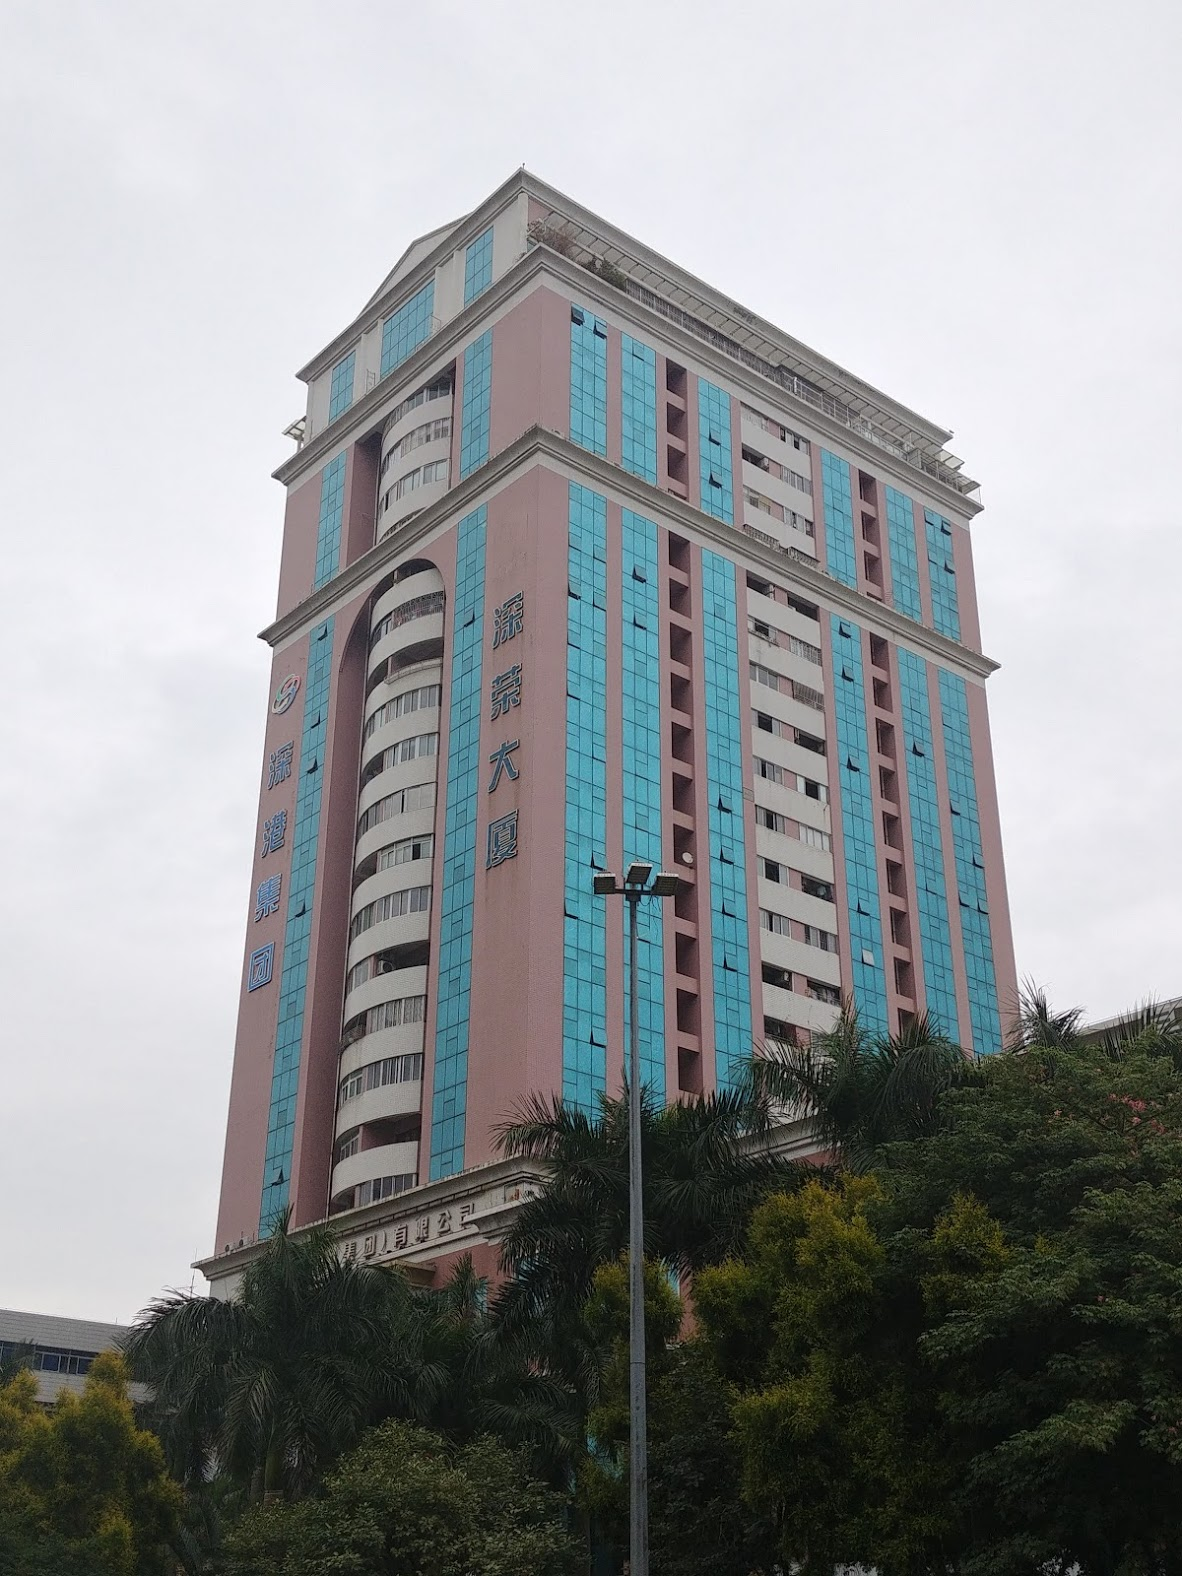
\includegraphics[scale=0.15]{figures/photos/photo_building.jpg}
\caption{Bureau à la frontière Chine - Hong-Kong}
\label{fig:photo_building}
\end{figure}

% TODO: add a screenshot of Maps

\chapter{Objectifs et contexte}
Mon stage s’est déroulé dans le pôle recherche et développement de Neohm, sous la direction de David \bsc{Collardeau}. Au début, nous étions 4 à travailler dans ces bureaux : David, Sy et Green et moi. Jean venez dans les bureaux environs une fois toutes les 2 semaines pour faire un point sur l'avancement et préparer au mieux l'industrialisation du produit. Plus tard, 2 nouveaux collaborateurs se sont ajoutés à l’équipe.
Le sujet initial du stage dont David m’avait parlé par téléphone en juillet était le projet « Looping », il s’agissait d’un chauffe biberon sur batterie utilisant le phénomène d’induction. Un élément chauffant en métal est placé dans un biberon rempli, le tout est placé sur ou dans le système de chauffe (selon le prototype).

\begin{figure}[H]
\centering
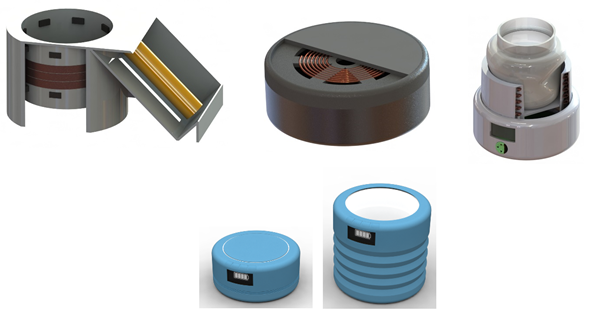
\includegraphics[scale=0.75]{figures/screenshots/3D_drawing_looping.png}
\caption{Dessins 3D de prototypes de Looping}
\label{fig:3D_looping}
\end{figure}

Guillaume, le directeur marketing basé en France est à l’origine du projet. Il a travaillé plusieurs années dans l’industrie du bébé avant de fonder Neohm, et selon lui il y aurait un fort potentiel pour une tel produit.
Cependant, après plusieurs semaines de travail sur ce projet durant l’été 2017, David s’est aperçu que la chauffe à induction comporte de nombreux défis techniques comme la modulation du courant envoyé dans les bobines ou l’isolation du système pour son champ électromagnétique n’interfère pas avec d’autres appareils électroniques. Le rendement de l’induction n’est pas non plus particulièrement bon, l’intérêt de cette technologie est la vitesse de chauffe car seul l’élément chauffant reçoit directement l’énergie.
L’équipe a donc décidé de mettre Looping et la chauffe par induction de côté pour se concentrer sur un autre projet : \emph{EasyFeed}. Ce projet est un système portatif qui permet à lui seul de confectionner un biberon. L’utilisateur y insère le lait en poudre et l’eau et le système remplit un biberon chaud avec les doses adaptées. L’eau sera ici chauffée par une simple résistance.
Mon travail sera de programmé le microprocesseur présent dans le produit qui contrôle les différentes fonctionnalité (affichage, contrôle de moteurs, charge des batteries, protections en température du produit…).

\chapter{Démarches et travaux réalisés}
\section{Looping / EasyFeed}
Au début du stage, David m’annonce que je commencerai à travailler sur la gestion des batteries dans \emph{EasyFeed}.
Dans un premier temps, il me demande de m’intéresser sur l’USB type C. Il veut équiper le produit d’un tel connecteur. Cette nouvelle norme permet d’unifier toutes les connecteurs USB en un seul.

\begin{figure}[H]
\centering
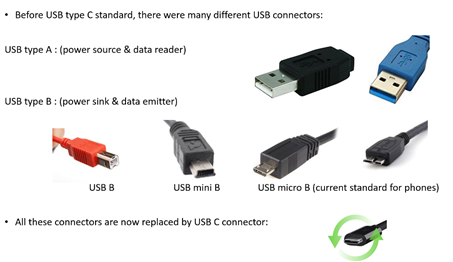
\includegraphics[scale=0.75]{figures/screenshots/different_usb_types.png}
\caption{Différents types de connecteurs USB}
\label{fig:usb_type}
\end{figure}

De plus, l’USB C est compatible avec la spécificité Power Delivery qui permet de fournir jusqu’à 100W de puissance électrique. Inclure l’USB C au produit apporterait un confort à l’utilisateur qui pourra par exemple utiliser le chargeur du MacBook d’Apple est un connecteur USB-C et qui fournit \SI{60}{\watt}.
L'USB C permet également un échange de donnée et de d'énergie dans les 2 sens du câble alors qu'auparavant, les données ne pouvait qu'aller du connecteur type B au connecteur type A et l'énergie du connecteur type B au connecteur type B (i.e. il n'était ni possible de changer un pc avec un portable et ni de lire des données d'un pc avec un portable).
Je me suis donc renseigné sur la norme USB Power Delivery qui peut en effet fournir jusqu’à 20V / 5A. Cependant, pour fournir une telle puissance, la source doit négocier la tension et le courant avec le débiteur de courant (figure~\ref{fig:usb_pd_negociation}).

\begin{figure}[H]
\centering
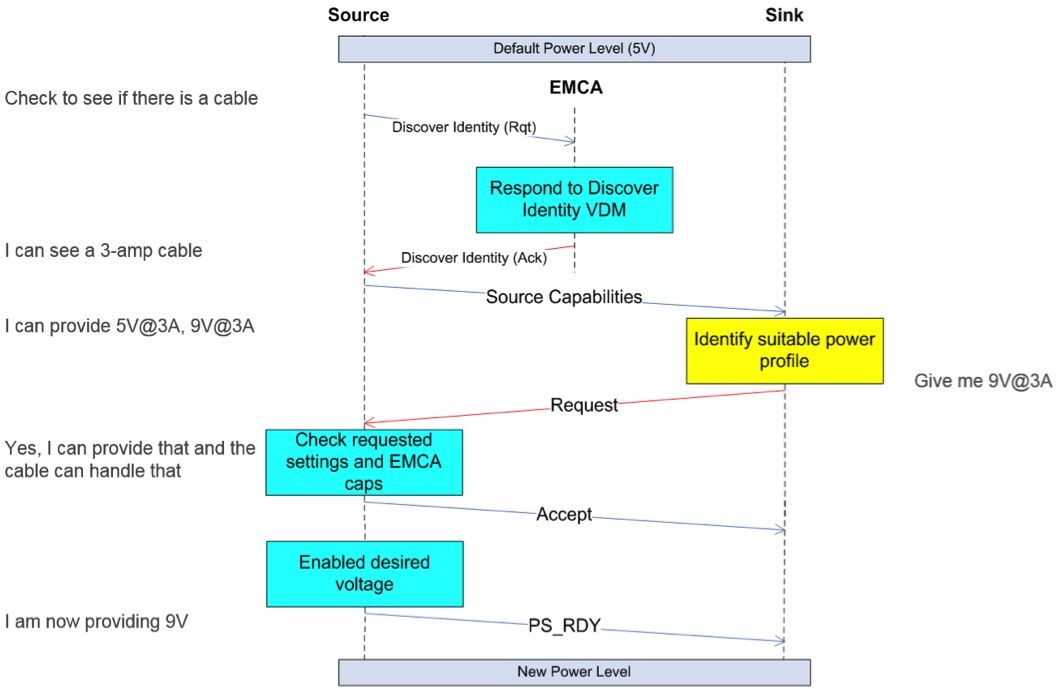
\includegraphics[scale=0.35]{figures/screenshots/usb_pd_nego.png}
\caption{Exemple d’une négociation USB PD (simplifiée) \cite{usb_pd_nego}}
\label{fig:usb_pd_negociation}
\end{figure}
% TODO: def of EMCA

Cette négociation nécessite un contrôleur spécifique. Les recherches que j’ai effectuées m’ont mené à des contrôleurs assez onéreux, environ 5\$/unité. De plus un adaptateur secteur / USB-C supportant \SI{80}{\watt} coûtent relativement cher car il s'agit d'une technologie nouvelle (notamment utiliser dans les derniers ordinateurs portables et téléphones)
Après avoir présenté mes recherches à David, il m'a présenté le PCB qu’il avait conçu (figure~\ref{fig:looping_pcb}) pour la gestion de l’alimentation du projet Looping car le pack batterie d'\emph{EasyFeed} allait être identique et les besoins d'alimentation semblables.

\begin{figure}[H]
\centering
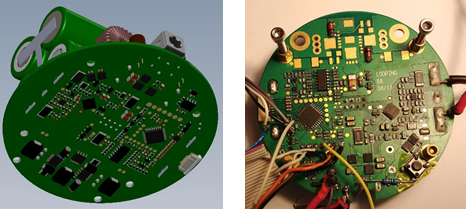
\includegraphics[scale=1]{figures/photos/looping_pcb.jpg}
\caption{PCB du projet Looping}
\label{fig:looping_pcb}
\end{figure}

Le circuit (figure~\ref{fig:looping_charger}) était conçu autour d'un contrôleur Texas Instrument BQ40Z60 gérant les phases de charges et de décharges du pack batterie et d'un microprocesseur Silabs 8 bits EFM8LB1 (pas présent sur le schéma) pour communiquer avec le contrôleur et de piloter globalement l'appareil (on/off, affichage du niveau de la batterie, boucle de contrôle de la température, ...).

\begin{figure}[h]
\centering
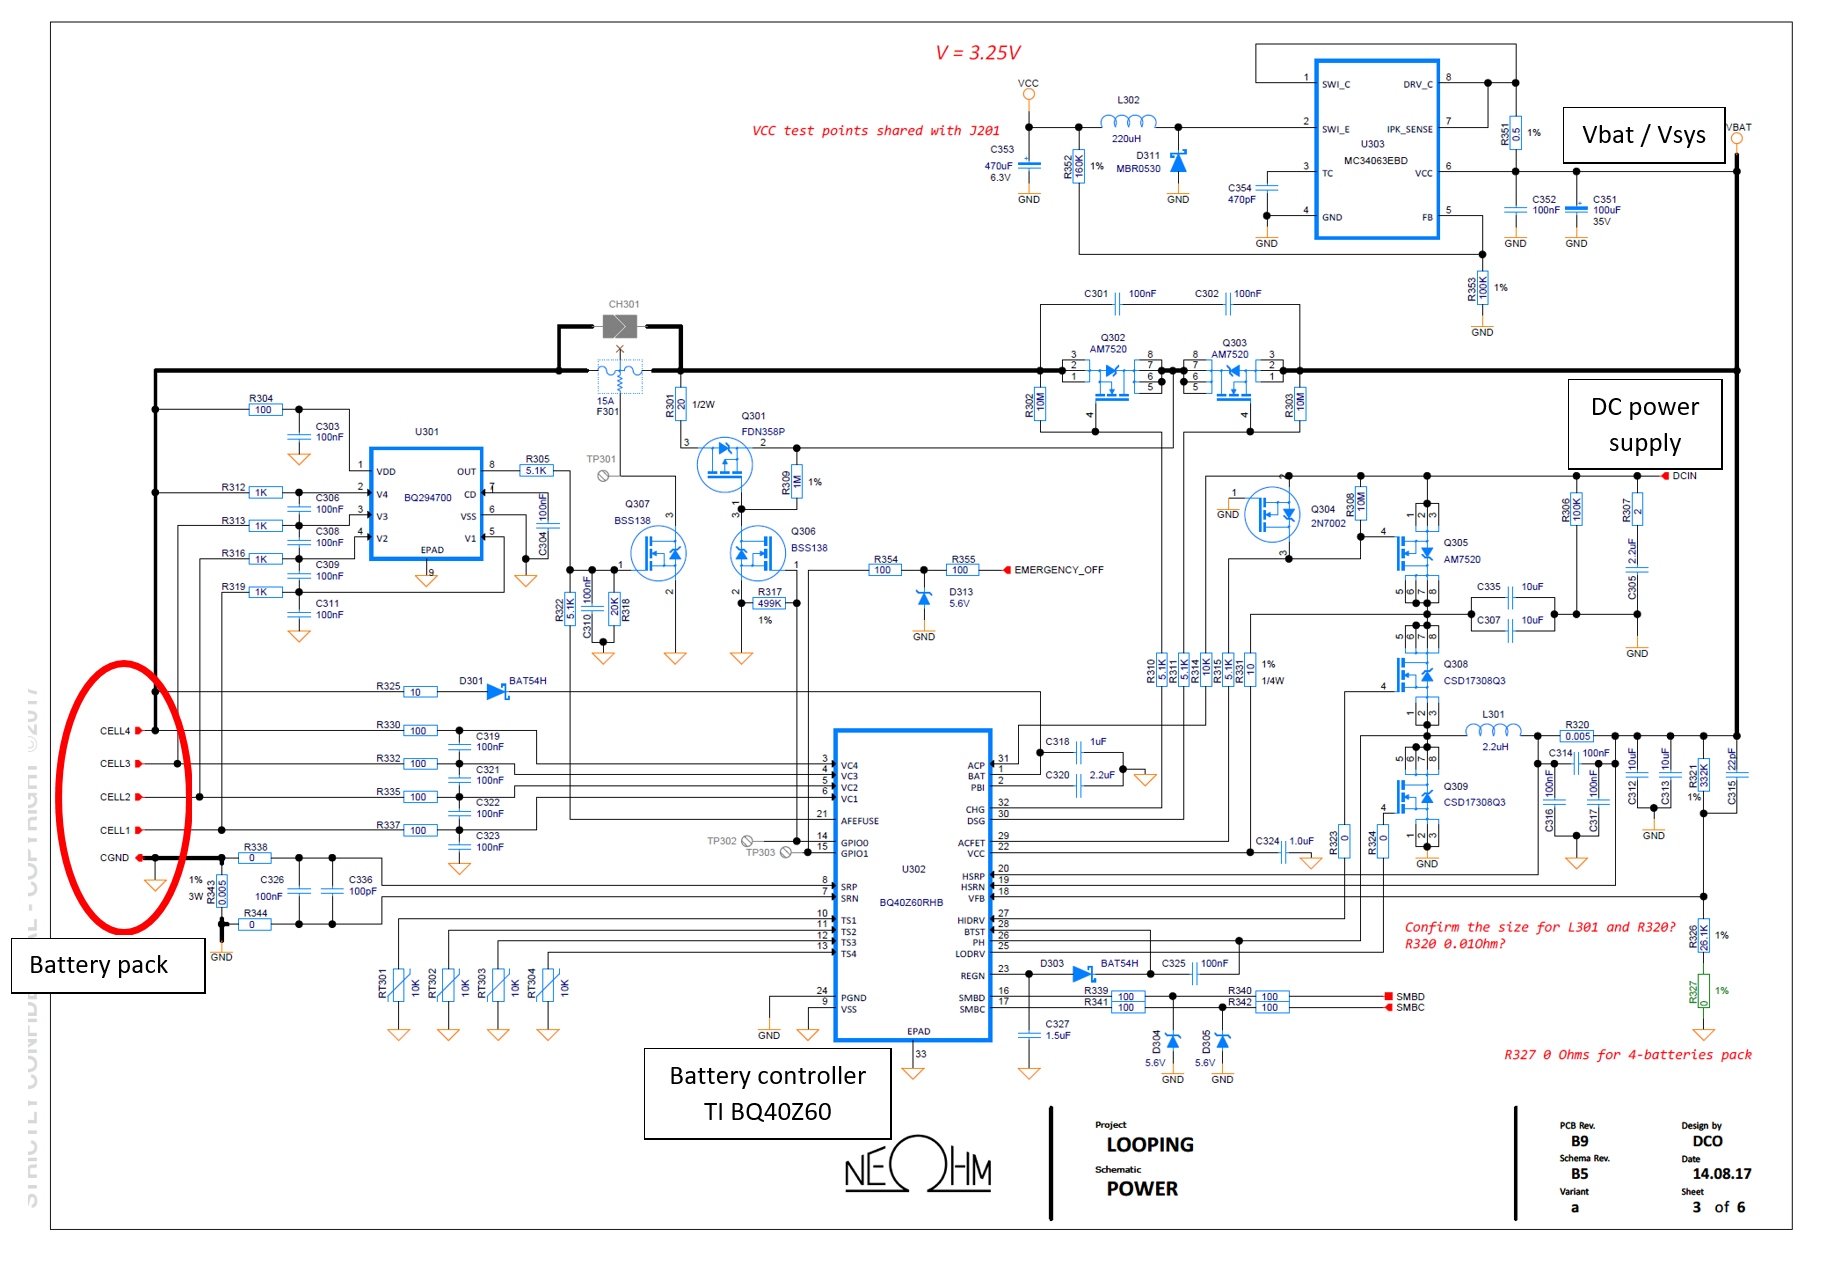
\includegraphics[scale=0.6]{figures/screenshots/battery_charger.png}
\caption{Schéma électrique de la gestion de batterie de Looping}
\label{fig:looping_charger}
\end{figure}

Mon travail fut donc de programmer le microprocesseur pour communiquer avec le contrôleur de batterie. J’ai dans un premier temps consulté attentivement les documentations et les manuels de ces 2 composants afin de comprendre leur fonctionnement. J’ai dû également m’intéresser au SMBus 
% TODO: ref to SMBus documentation
qui permet aux 2 puces de communiquer via les fils SMBD et SMBC.
Le composant BQ40Z60 gère à la fois la charge de la batterie, la décharge, l’équilibre des cellules, les protections en température et en courant, l’estimation du niveau de batterie. SMBus permet de configurer la puce et surveiller son état pendant son fonctionnement.
SMBus utilise donc 2 lignes pour communiquer :
\begin{itemize} % TODO: bullets instead of hyphen
\item SMBD est une ligne de données bidirectionnelle,
\item SMBC est une ligne d'horloge de synchronisation bidirectionnelle,
\end{itemize}

Pour visualiser le protocole SMBus, j’avais à disposition un oscilloscope pour observer un représentation des signaux électriques traversant les 2 lignes (figure~\ref{fig:SMBus_oscilloscope}) ainsi qu’un analyseur logique (figure~\ref{fig:SMBus_logic_analyser}).

\begin{figure}[H]
\centering
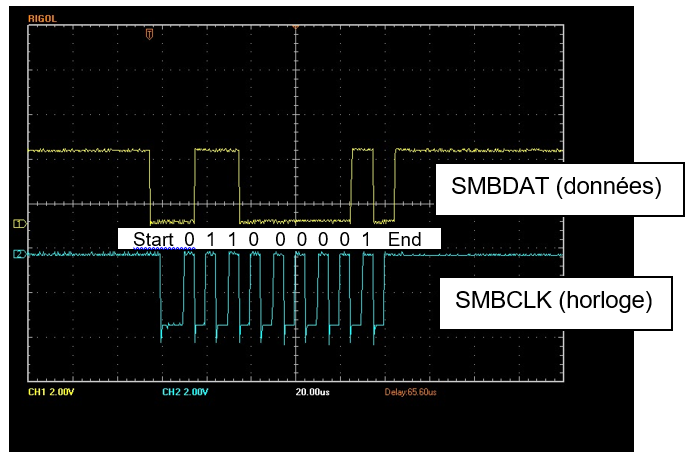
\includegraphics[scale=0.6]{figures/screenshots/SMBus_oscilloscope.png}
\caption{Byte SMBus visualisé avec un oscilloscope}
\label{fig:SMBus_oscilloscope}
\end{figure}

\begin{figure}[H]
\centering
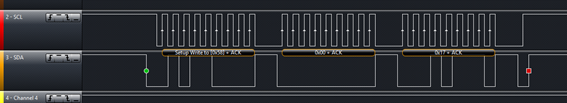
\includegraphics[scale=0.9]{figures/screenshots/SMBus_logic_analyser.png}
\caption{3 bytes SMBus visualisés avec un analyseur logique}
\label{fig:SMBus_logic_analyser}
\end{figure}

L’analyseur logique permet d’être plus rapide car il convertit les données directement en hexadécimal tandis que l’oscilloscope donne un représentation plus réaliste des signaux pour repérer des problèmes analogiques (signaux bruités, capacitifs) par exemple.
Le principal problème que j’ai rencontré est que le BQ40Z60 ne semblait pas piloter les 2 transistors FET qui gèrent la charge et la décharge de la batterie (les 2 transistors en série sur le schéma électrique).
J’ai donc essayer de contrôler ces transistors manuellement avec des commandes expliqué dans le manuel du composant (figure~\ref{fig:BQ40Z60_manual_excerpt}).

\begin{figure}[H]
\centering
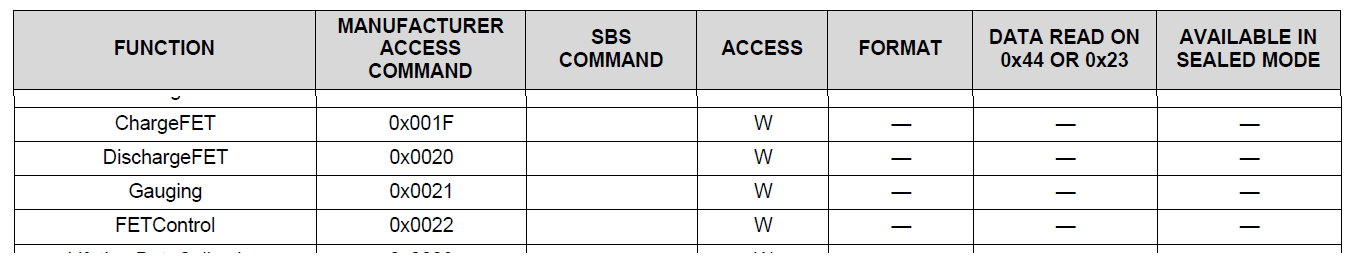
\includegraphics[scale=0.82]{figures/screenshots/BQ40Z60_manual_excerpt.png}
\caption{Extrait du \emph{BQ40Z60 Technical Reference Manual}\cite{BQ40Z60_tech_manual}} 
\label{fig:BQ40Z60_manual_excerpt}
\end{figure}

Le contrôleur ne semblait pas apprécier ces commandes car après avoir reçu celles-ci, il ne fonctionnait pas, il renvoyait un NACK au lieu d’un ACK puis plus aucune fonction ne répondait (comme la lecture du numéro de série du composant pas exemple).
J’ai fait part de mes difficultés à contrôler le composant à David, il a décidé de commander un débogueur spécifique pour les contrôleur batterie de Texas instrument, le EV2300. Cette appareil fonctionne avec le logiciel BQStudio (figure~\ref{fig:BQ40Z60_registers}) qui propose une interface permettant de visualiser tous les registres du BQ40Z60 et le configurer plus aisément. Ce projet a été mis en pause en attendant de recevoir ce débogueur.

\begin{figure}[H]
\centering
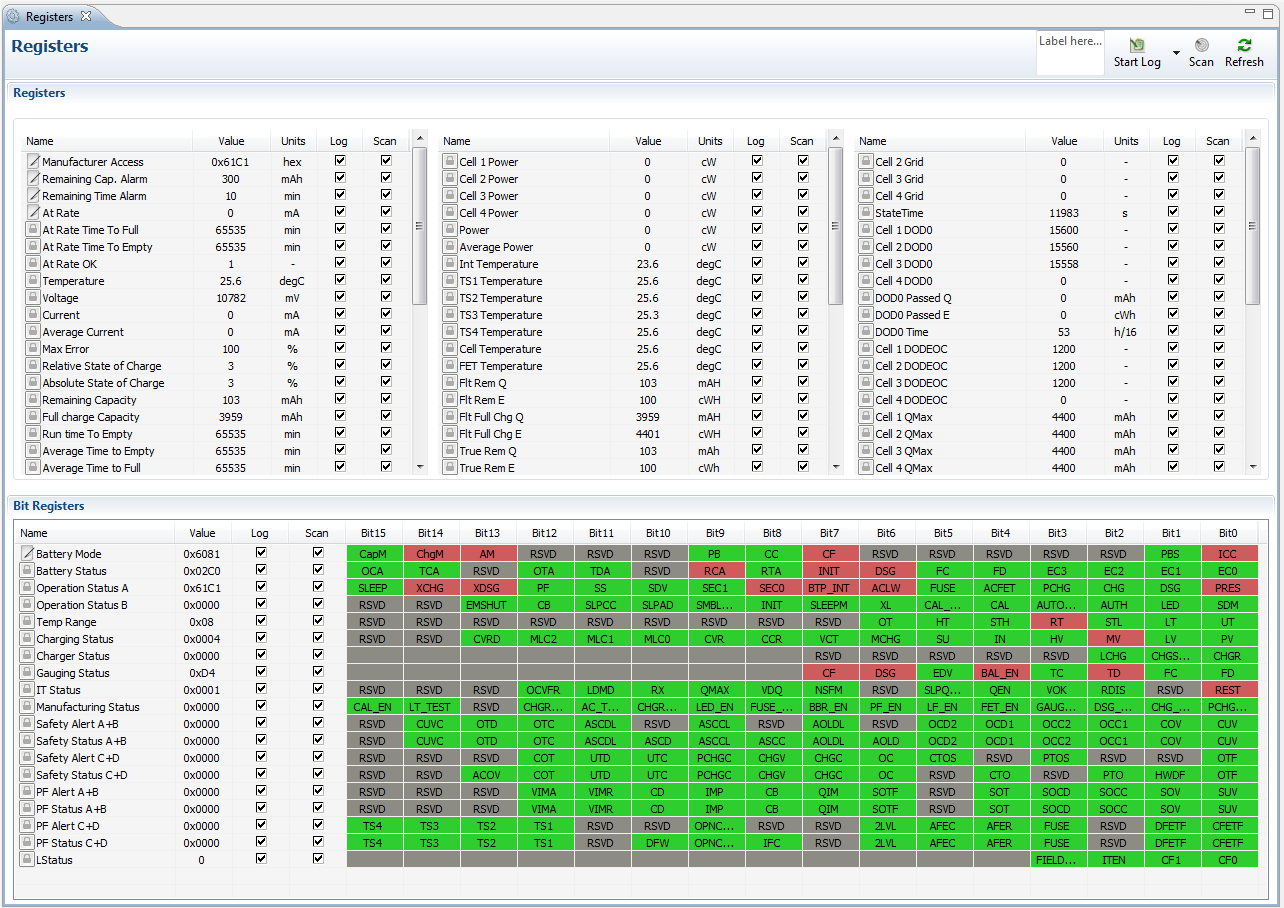
\includegraphics[scale=0.4]{figures/screenshots/BQ40Z60_registers.png}
\caption{Registres du BQ40Z60 dans le logiciel BQ studio}
\label{fig:BQ40Z60_registers}
\end{figure}

\section{Site web}
En parallèle de ce projet, Guillaume, le directeur marketing de la start-up, m’a demandé d’adapter le site internet \url{neohm.net} fraîchement créé par David pour qu’il soit correctement visible sur mobile.
Le site internet avait conçu à partir d’un template du framework Bootstrap. Il était donc à 90\% adapter pour mobile mais il fallait corriger quelques défauts. J’ai donc modifier dans le feuille de style la taille de certains éléments en utilisant une technologie \emph{responsive} qui s’adapte à la taille de l’écran, modifier la position de conteneurs d’absolue à relatif et ajuster certaines marges qui faisait apparaître une barre de défilement horizontale sous mobile. J’ai également modifier le code JavaScript d’une fonction qu’avait rajouté David, qui permet d’afficher périodiques des mots sur une image de fond pour que cela fonctionne également sur smartphone. Après ces modifications, le site était parfaitement lisible depuis tout appareil (figure~\ref{fig:website}).

\begin{figure}[H]
\centering

\includegraphics[scale=0.25]{figures/screenshots/website.png}
\caption{Avant/après du site vu d’un smartphone}
\label{fig:website}
\end{figure}

\section{Serveur}
David a décidé de mettre en place un serveur au bureau afin de centraliser les projets, les ressources, l’impression. Sy, l’ingénieur chinois, s’est chargé de monter le serveur, d’y installer Linux Ubuntu et de mettre en place le logiciel Samba pour partager des dossiers et l’imprimante en réseau local. Ma mission fût de créer un accès distant au serveur via le protocole FTP. J’ai installé le paquet VsFTPd afin de créer un serveur sécurisé. Le problème est que l’adresse IP de la connexion internet attribuer par notre fournisseur d’accès n’est pas fixe, et demander un IP fixe coûte cher en Chine. Pour parer ce problème, David m’a demandé d’installer le logiciel TeamViewer qui permet de prendre le contrôle d’un PC à distance via une connexion internet. Ainsi, pour se connecter au serveur FTP à distance, il faut dans un premier temps utiliser TeamViewer afin de déterminer l’adresse IP actuel du serveur, puis utiliser un client FTP pour se connecter aux serveurs.
David m’a également chargé de mettre en place un gestionnaire centralisé de gestion version. J’ai donc installé Apache Subversion sur le serveur. Travailler avec un tel gestionnaire permet d’être plus efficace en équipe et assure une traçabilité des modifications effectuées sur les projets.
A la demande de l’équipe, je me suis occupé de trouver un moyen pour contourner le pare-feu chinois qui nous empêche l’accès à de nombreux sites utiles dans notre travail : Google, Gmail, WhatsApp, YouTube, etc. 2 solutions s’offraient à moi : mettre en place un VPN sur un router wi-fi ou utiliser le réseau 4G hongkongais que l’on capte dans les locaux (proche de la frontière avec Hong-Kong) pour fournir l’accès internet. Je suis allé à Hong-Kong afin de me renseigner et d’acheter un router wi-fi compatible. Sur les conseils d’un vendeur, j’ai choisi un router à la fois compatible avec les VPN et avec une clé USB 4G (figure~\ref{fig:wifi_router}).

\begin{figure}[H]
\centering
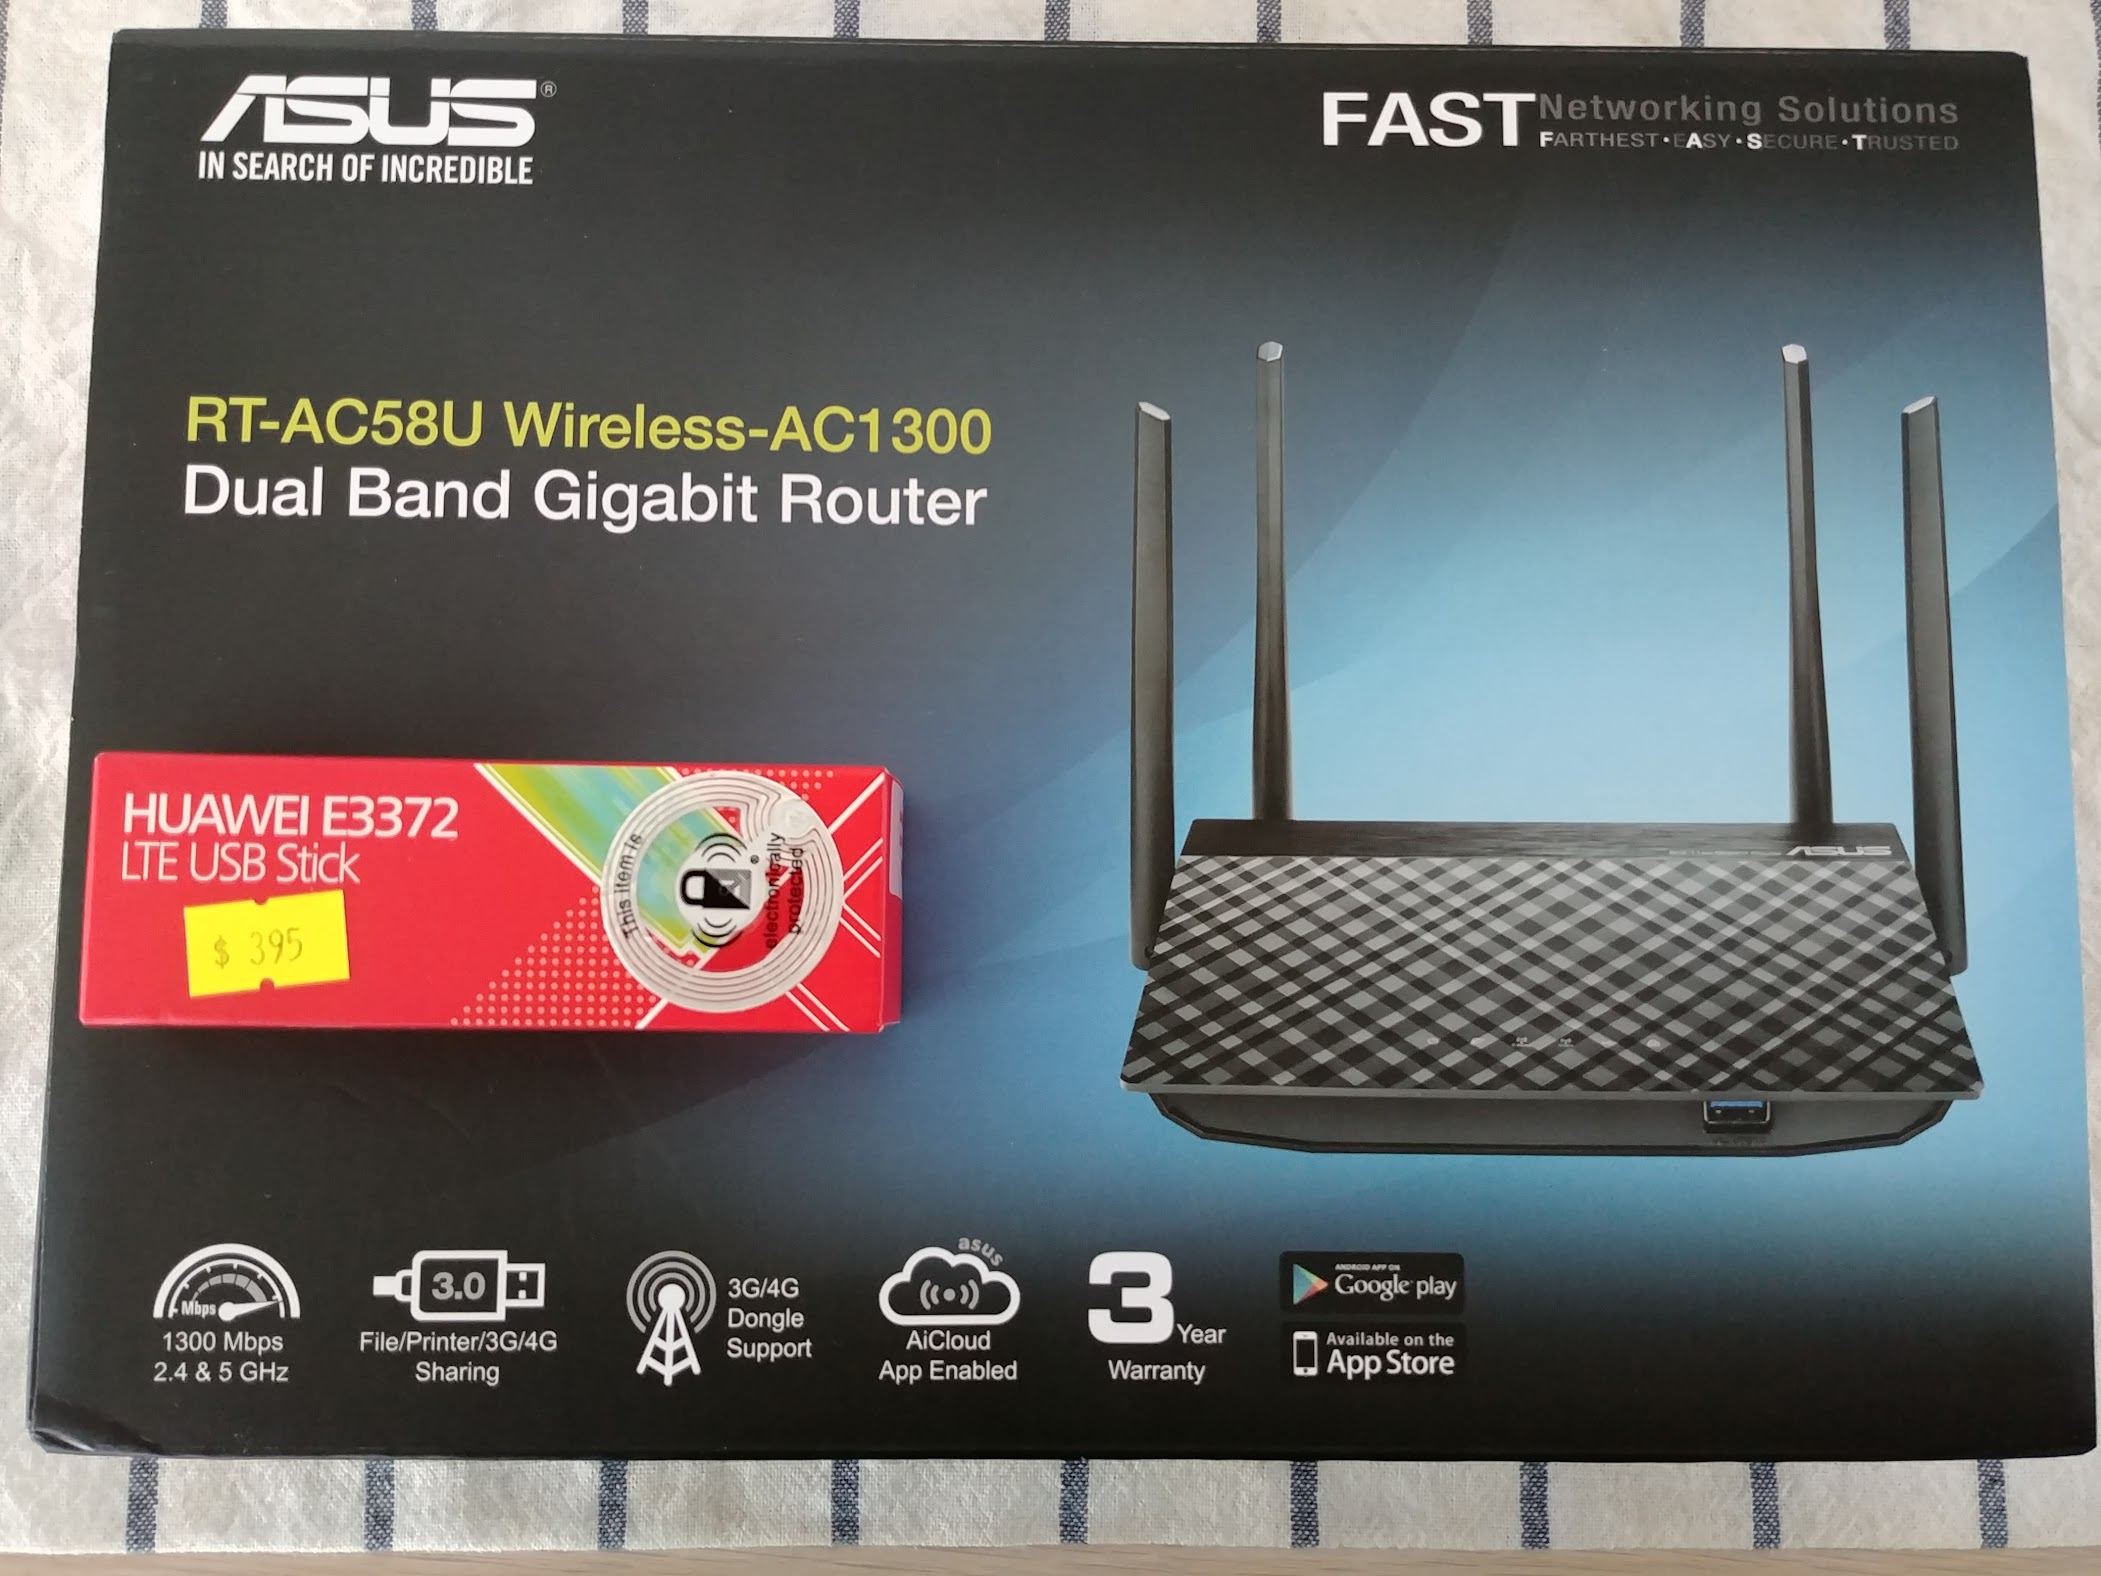
\includegraphics[scale=0.12]{figures/photos/wifi_router.jpg}
\caption{Router wi-fi compatible VPN avec une clé USB LTE}
\label{fig:wifi_router}
\end{figure}

\section{Worklamp}
\subsection{Présentation}
David m’a présenté un autre projet en cours sur lequel j'allai travailler : une lampe à LED portable pour peintre. Cette lampe existe sous 2 versions : une version \emph{AC} \SI{80}{\watt} alimentée par le secteur et une version \emph{DC} \SI{50}{\watt} alimentée par batterie. Pour simplifier l'industrialisation du produit, le boîtier est identique pour les 2 versions mais tous les ports ne sont utilisés dans chaque version (figure~\ref{fig:captioned_worklamp}). Le PCB et le panneau de LEDs sont quand à eux spécifiques à chaque version du produit (figure~\ref{fig:worklamp_PCBs}). Il y a plus de LEDs dans la versions \SI{80}{\celsius} et les PCBs n'ont pas le même rôle (redressement et lissage de la tension pour la version AC, gestion de la batterie pour la version DC).
Dans les 2 version, un potentiomètre permet de faire varier lumineuse. Les panneaux de LEDs sont composés de 2 types de LEDs (\SI{3700}{\kelvin} et \SI{5700}{\kelvin}) afin de disposer de 3 modes d’éclairage différents. Un bouton permet de changer la température de la couleur émise : \SI{3700}{\kelvin}, \SI{5700}{\kelvin} et \SI{4200}{\kelvin} (les 2 types de LEDs sont allumés à mi-puissance). 

\begin{figure}[H]
\centering
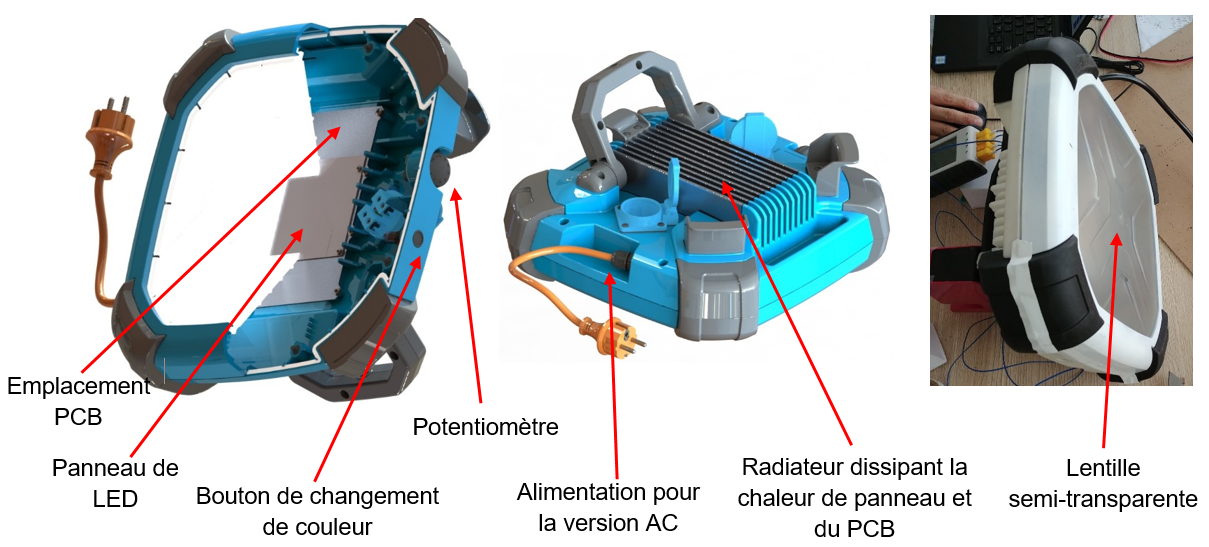
\includegraphics[scale=0.45]{figures/screenshots/captioned_worklamp.png}
\caption{Dessin 3D et photo de la worklamp}
\label{fig:captioned_worklamp}
\end{figure}

\begin{figure}[H]
\centering
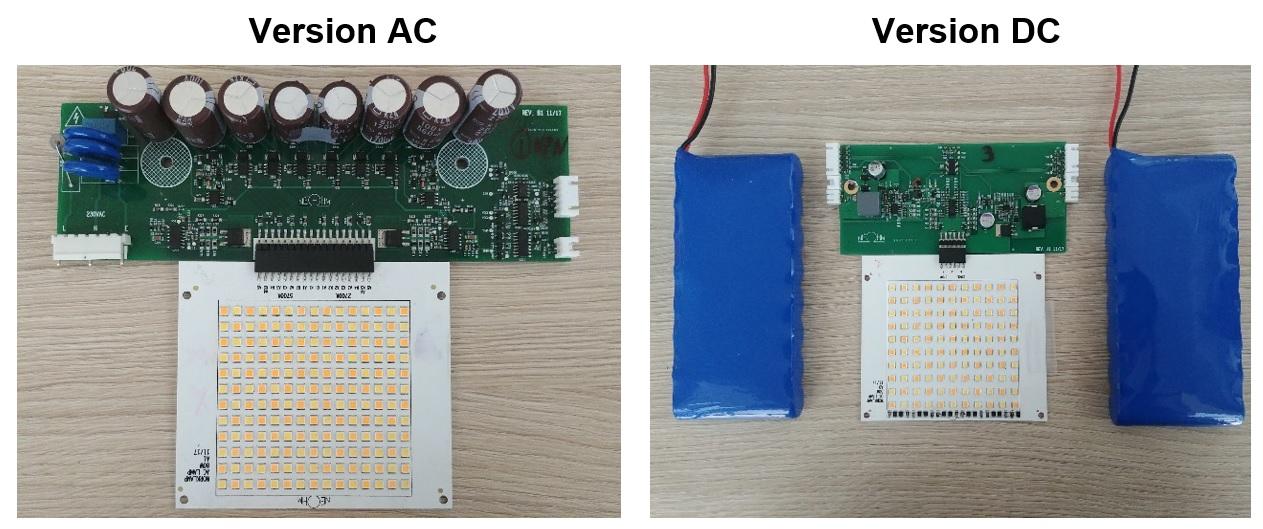
\includegraphics[scale=0.43]{figures/photos/worklamp_PCBs.jpg}
\caption{PCBs des versions AC et DC de la worklamp}
\label{fig:worklamp_PCBs}
\end{figure}

Ma mission a porté sur la version DC, j’ai été en charge de la programmation du microprocesseur présent dans le circuit, du débogage et des tests les prototypes. La version AC est purement hardware, elle est composée de filtres analogiques et de bascules pour gérer le changement de mode de couleur. A contrario, la version DC comporte un processeur pour pouvoir gérer le pack batterie (charge, état du niveau de batterie, protection en courant et température) et nécessite donc un développement logiciel. Le langage de programmation utiliser était le C.

\subsection{Schéma électrique}
David m’a donc transmis le schéma électrique (figure~\ref{fig:worklamp_schema}) qu’il avait conçu qui correspond au PCB du modèle DC pour que je me l’approprie pour ensuite implémenter un software dans le microprocesseur.

\begin{figure}[H]
\centering
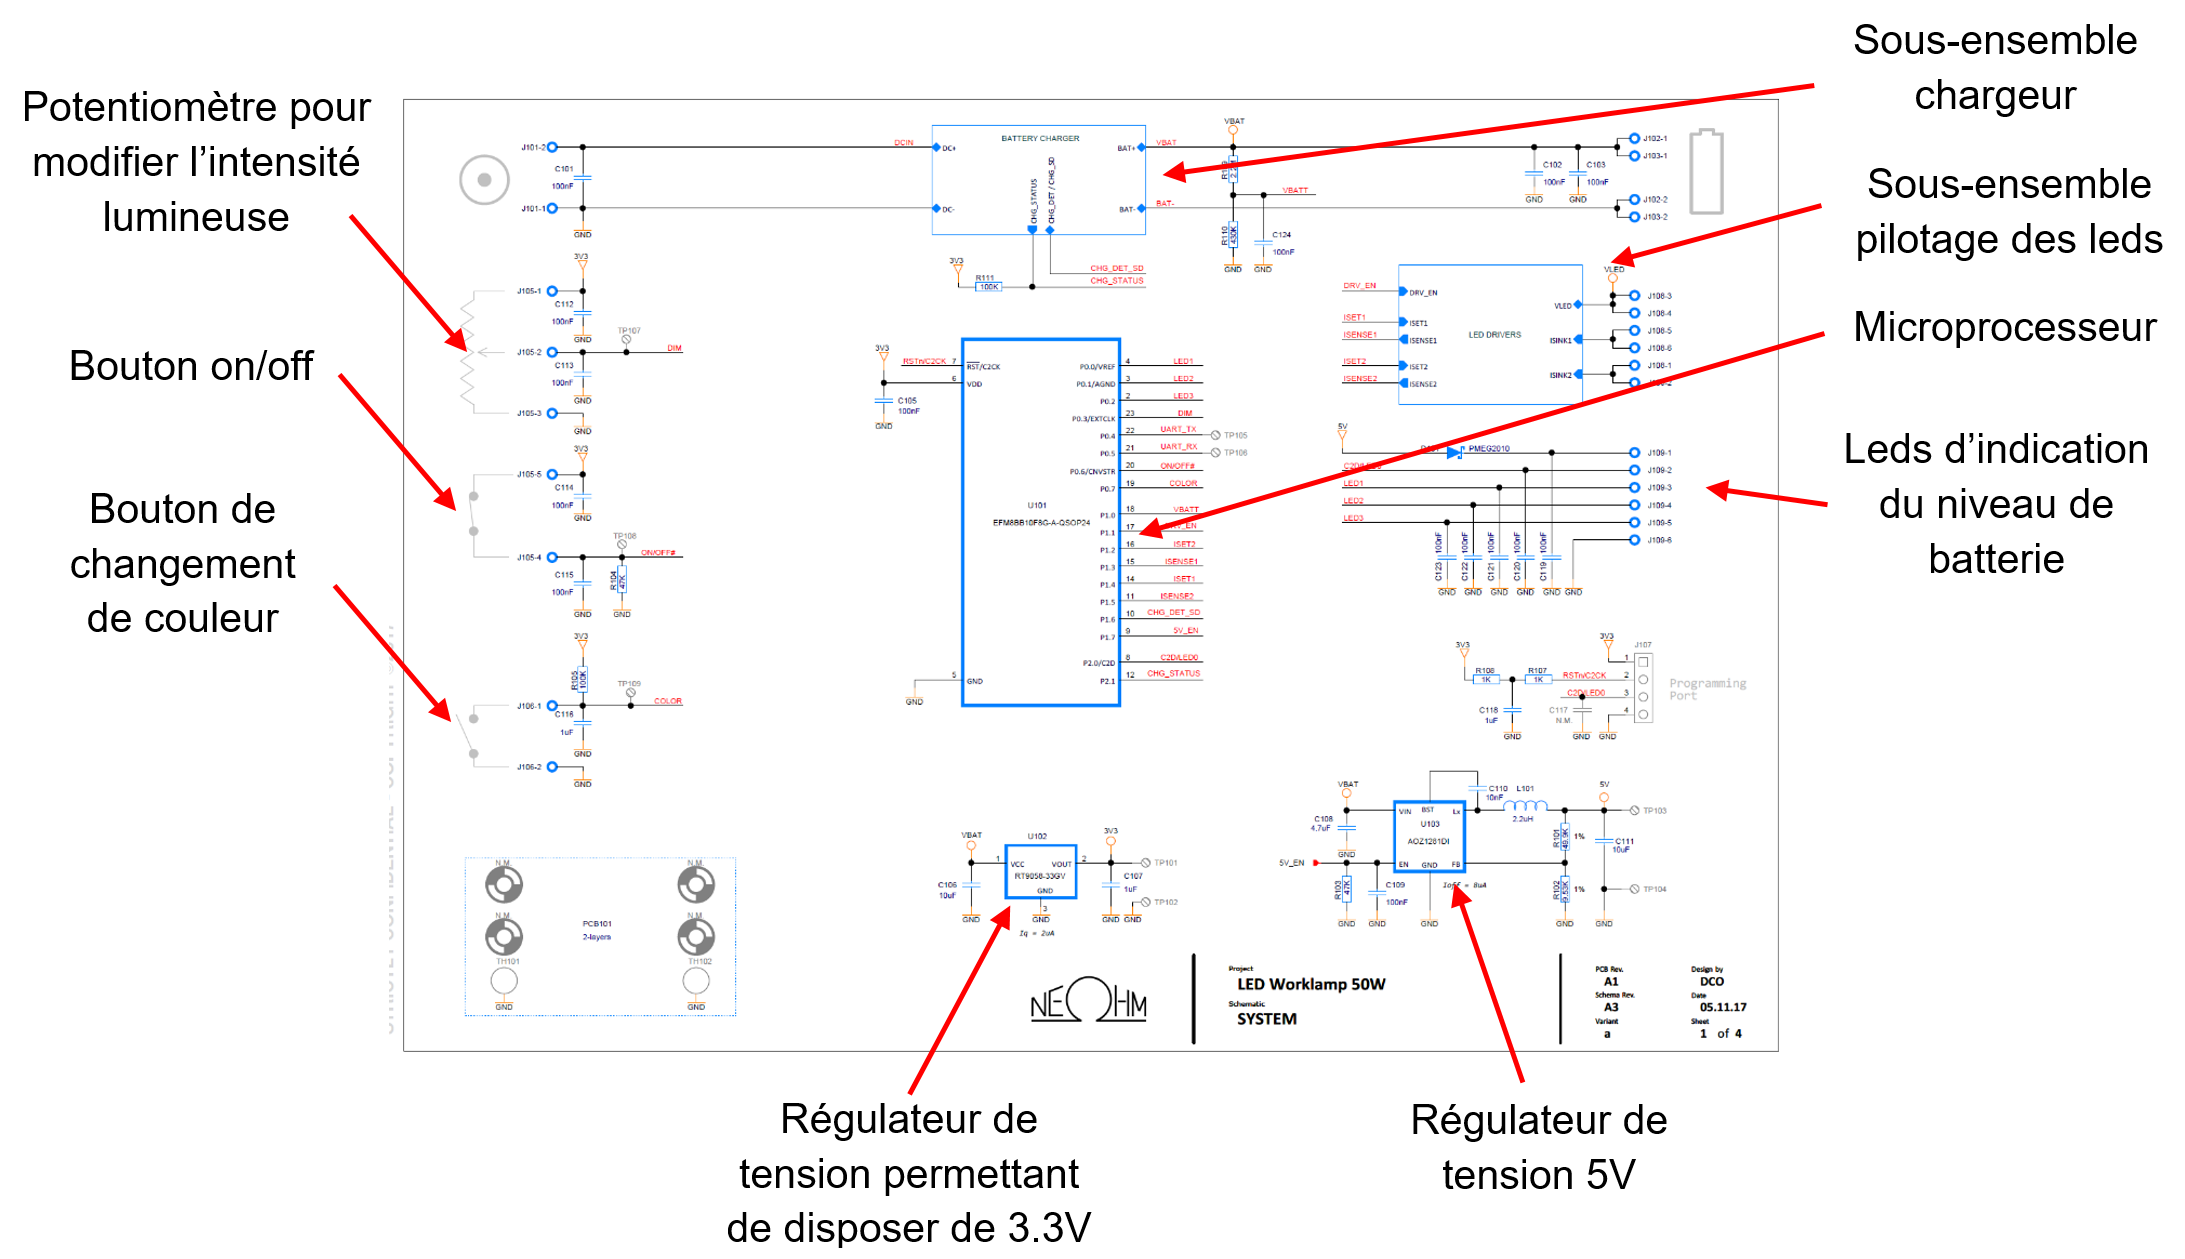
\includegraphics[scale=0.51]{figures/screenshots/version_A3_worklamp.png}
\caption{Schéma électrique de la Worklamp}
\label{fig:worklamp_schema}
\end{figure}

La première étape fut d’écrire une spécification pour définir les tâches à remplir par le processeur pour ensuite aboutir à un ensemble d’algorithme accomplissant ces missions.
Les tâches que doit effectuer le processeur sont :
\begin{itemize} % TODO: bullets instead of hyphen
\item Se mettre en veille (mode basse consommation) sur commande du bouton ON/OFF,
\item Moduler l’intensité lumineuse en fonction de l’état du potentiomètre,
\item Changer la couleur sur un appui sur le bouton COLOR,
\item Indiquer l’état de charge des batteries quand la lampe est en fonctionnement ou en charge à l’aide de 4 LEDs,
\item Fournir un port USB de charge 5V lorsque la lampe n’est pas en veille,
\item Gérer la charge du pack batterie,
\item Protéger le produit en cas de surchauffe.
\end{itemize}


Il a ensuite fallu de définir la configuration des pins du microprocesseur en accord avec le schéma grâce la datasheet du EFM8BB1 (figure~\ref{fig:pins_definition}). Il s’agit de définir des fonctions et noms variables aux différents pins (input, output, PWM, ADC, UART, SMB, …).

\begin{figure}[H]
\centering
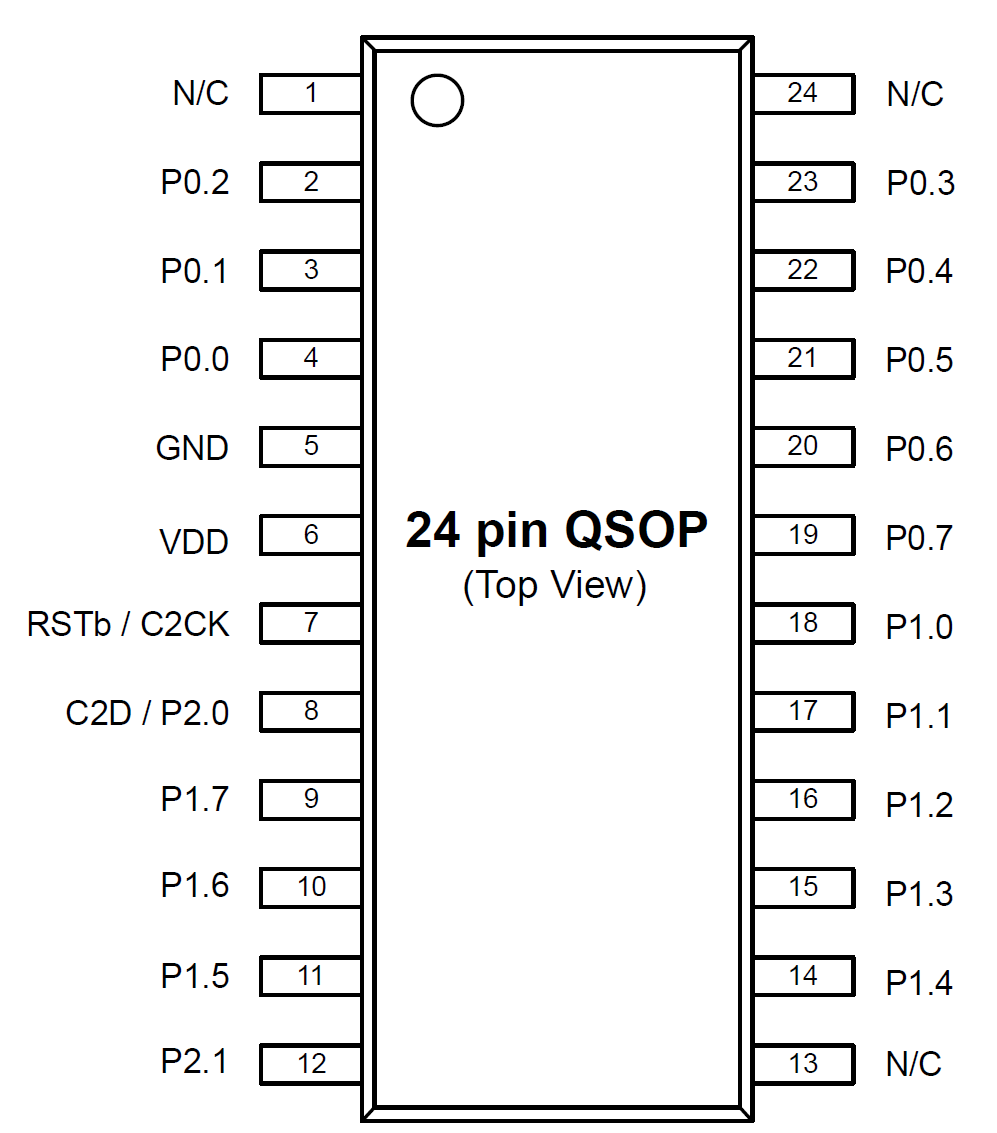
\includegraphics[scale=0.4]{figures/screenshots/pins_definition_EFM8BB.png}
\caption{Définition de pins sur le processeur EFM8BB1x-QSOP24\cite{EFM8BB1_datasheet}}
\label{fig:pins_definition}
\end{figure}

Cette étape est cruciale pour la suite du développement et demande quelques notions d’électronique. Par exemple il faut définir si le pin est défini en \emph{open drain}, c’est-à-dire que l’état haut correspond à une forte impédance et l’état bas à une faible impédance, ou en \emph{push-pull}, si l’on veut que l’état haut soit le \SI{3.3}{\volt} du CPU, et état bas du CPU (figure~\ref{fig:opendrain_pushpull}). 

\begin{figure}[H]
\centering
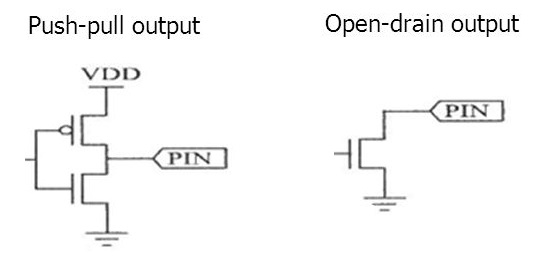
\includegraphics[scale=0.55]{figures/screenshots/opendrain_pushpull.png}
\caption{Illustration sortie \emph{Open drain} et \emph{Push-pull}} 
\label{fig:opendrain_pushpull}
\end{figure}

\subsection{Charge}
Le pack batterie est composé de 2 batteries lithium-ion 4S (tension nominal $4\times3,7=\SI{14.8}{\volt}$) en parallèle pour une capacité totale de \SI{10.4}{\ampere\hour} (\SI{153.92}{\watt\hour}). En fonction de l’avancement du projet, on a changé de contrôleur gérant la charge de la batterie, on est passé du BQ2000 au BQ25703A qui est plus performant et qui nous permet qui directement lire la tension de la batterie pour estimer son état de charge et de surveiller le courant de charge/décharge via la protocole I2C.

Un contrôleur pour charger la batterie lithium-ion permet de gérer les 3 phases de la charge. La dernière phase est la \emph{trickle charge}, elle est optionnelle et permet d’optimiser la durée de vie de la batterie si celle-ci a un très bas niveau, tous les contrôles n’intègre pas cette phase. Durant la \emph{trickle charge}, un faible courant est transmis à la batterie afin d’atteindre une certaine tension. La 2\ieme{} phase est le \emph{constant current} : un courant élevé est envoyé dans le pack batterie jusqu’à atteindre la tension de charge. Dans mon cas, le courant est de $2\times2,6 = \SI{5.2}{\ampere}$ (2 packs en parallèle) et la tension de charge de $4\times4,2 = \SI{16.8}{\volt}$ (chaque pack à 4 cellules en série). La dernière phase est le \emph{constant voltage} : on fixe une certaine tension (\SI{16.8}{\volt} dans mon cas) aux bornes du pack batterie jusqu’à atteindre un certain courant, puis on garde cette tension pendant \SIrange{30}{60}{\minute} pour finaliser la charge.

Bien que cet algorithme est implémenter dans les contrôleurs gérant la charge de batterie, sa compréhension était indispensable car j'ai dû vérifier que les différents circuits le respecter bien. Pour ce faire, après avoir vidé une batterie suite à une série de test, j'activais le circuit de charge et je vérifiais que les différentes étapes étaient respectées. Si le contrôleur était mal utilisé, la tension de charge pouvait trop haute ou trop basse, ce qui présente un danger pour la batterie et sa durée de vie.



\begin{figure}[H]
\centering
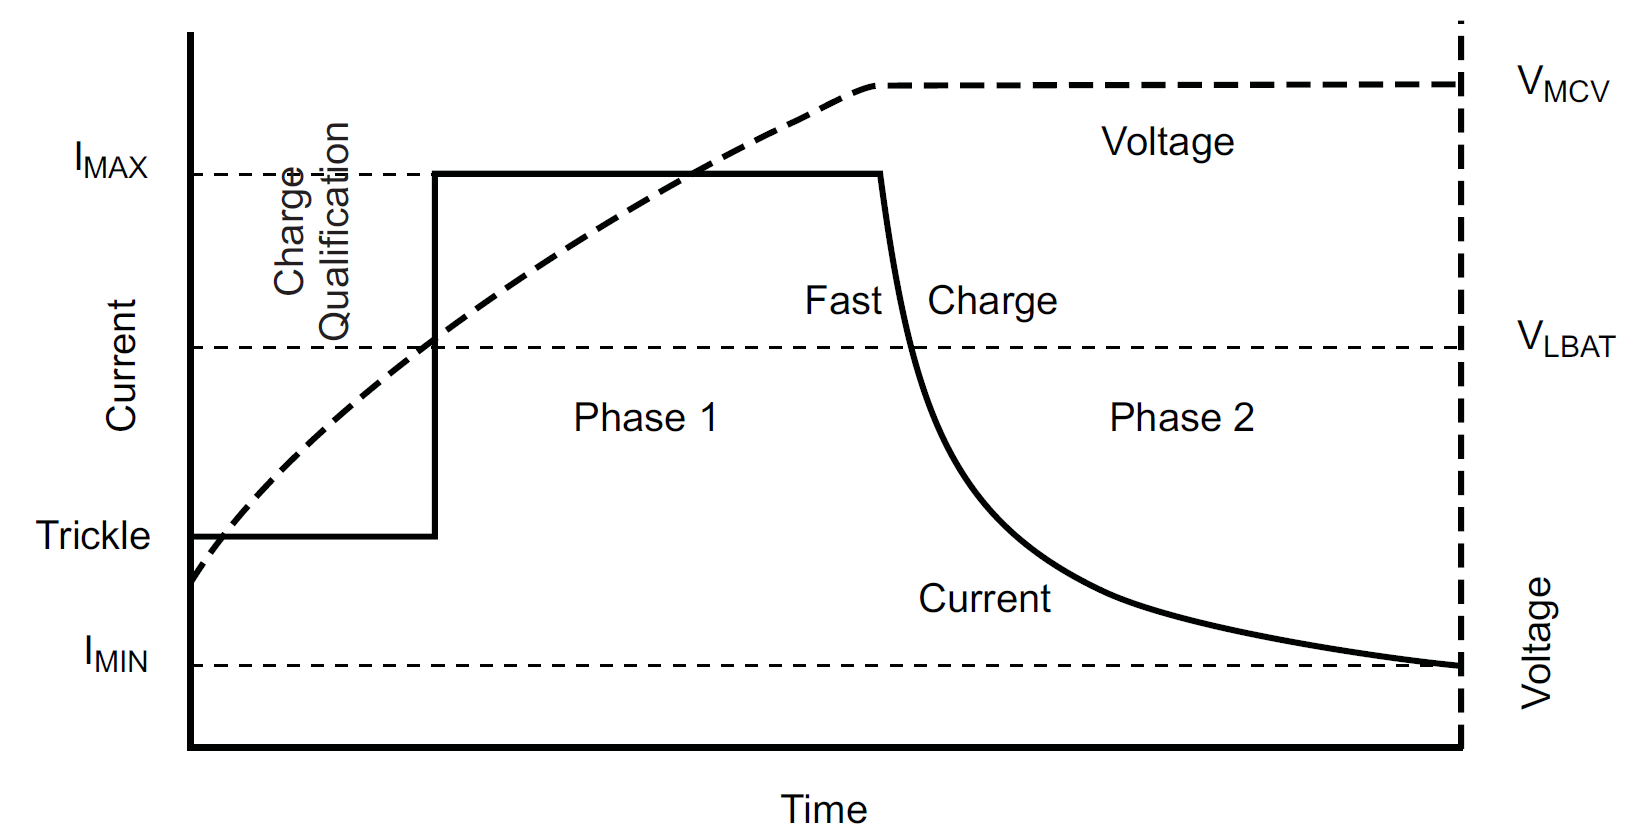
\includegraphics[scale=0.65]{figures/screenshots/Li-ion_charge_algortihm.png}
\caption{Algorithme de charge d’une batterie lithium-ion \cite{BQ2000_datasheet}} 
\label{fig:li-ion_charge}
\end{figure}

\subsection{Software}
J'ai conçu des algorigrammes pour chaque fonctionnalité que le Software doit gérer (figure~\ref{fig:flow_chart}). Cette étape m'a permis d'avancer dans le développement logiciel en gardant un certain recul avec les consignes auxquelles je m'étais fixé.

J'ai dû faire face aux contraintes de l'embarqué en concevant mon code. Il fallait notamment paramétrer le processeur pour donner les rôles de chaque broche (ADC, PWM, ...). La documentation du processeur expliquait comment utiliser des registres pour paramétrer les registres. 

\begin{figure}[H]
\centering
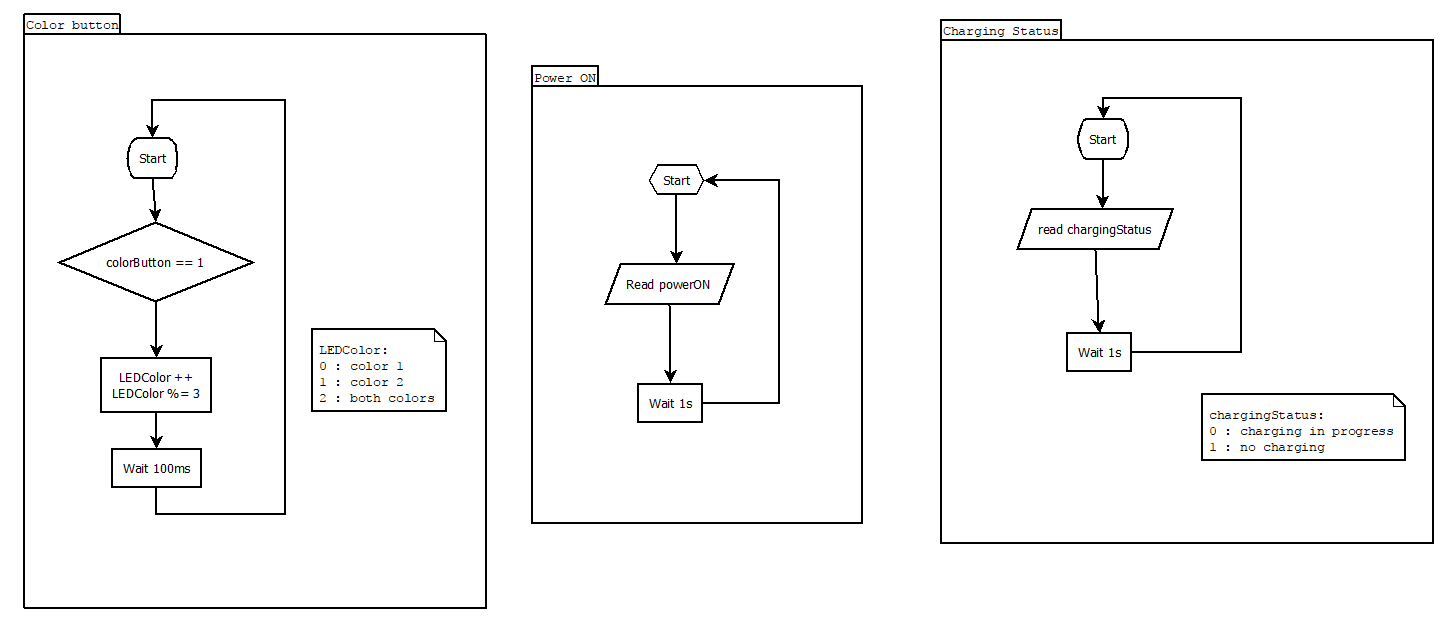
\includegraphics[scale=0.7]{figures/screenshots/flow_chart.png}
\caption{Quelques algorigrammes du software de la worklamp} 
\label{fig:flow_chart}
\end{figure}

\subsection{Tests}
A chaque étape du développement du la worklamp, le prototype a dû  être tester pour pouvoir évaluer la pertinance des solutions adoptées. Plusieurs mesures ont été effectuées sur un certain intervalle de temps pour vérifier si la lampe validait les critères imposés par le client dans le cahier des charges.
\begin{itemize} % TODO: bullets instead of hyphen
\item La température à l'extérieur du produit (au point le plus chaud, au niveau du radiateur passif) devait être inférieur à \SI{50}{\celsius} pour que l'utilisateur ne se brûle pas en utilisant la lampe (norme de sécurité européenne),
\item La température à l'intérieur du produit au niveau du PCB et du panneau de LEDs devait rester inférieure à certaines valeurs données dans les datasheets des composants pour assurer le bon fonctionnement de ces derniers (généralement \SIrange{70}{80}{\celsius}),
\item La tension et le courant au niveau du pack batterie et du panneau de LED étaient mesurés afin d'estimer le rendement du PCB (90\% minimum),
\end{itemize}
La mesure de la puissance électrique envoyée au panneau de LEDs multipliée par le rendement des LEDs données par le constructeur permet d'obtenir une bonne estimation de la puissance lumineuse émise. Le rendement global du produit ainsi que le temps d'utilisation du produit (5h minimum) pouvait donc être calculé.

La plupart des tests ont été réaliser dans les bureaux de Neohm. Des lunettes spécifiques étaient à notre disposition pour protéger nos yeux. En effet, la lumière émise, même à faible intensité, était aveuglante (figure~\ref{fig:lamp_with_glasses}).

\begin{figure}[h]
\centering
\includegraphics[scale=0.08]{figures/photos/tests_worklamp/lamp_with_glasses.jpg}
\caption{Panneau de LEDs en mode \SI{5700}{\kelvin} et \SI{4200}{\kelvin} à travers les lunettes de sécurité}
\label{fig:lamp_with_glasses}
\end{figure}

Pour mesurer plus précisément la puissance lumineuse émise (la lentille semi-transparente était ignoré dans le modèle ci-dessus) et pour obtenir la température (en Kelvin) émise, mon collègue Green et moi-même avons été dans un laboratoire spécialisé dans les lampes à LEDs équipé d'une \emph{sphère intégrante}. Cette appareil est un sphère blanche de 1m de diamètre dans laquelle on place la lampe à tester. Les capteurs sont reliés à une grande armoire électrique elle-même connectée à un ordinateur.

Ces tests étaient particulièrement pertinents pour la température de la lumière créé. En effet, dans le mode intermédiaire (\SI{5700}{\kelvin}). J'avais programmé le processeur pour envoyer 50\% de la puissance électrique dans les LEDs à \SI{6700}{\kelvin} et 50\% dans les LED à \SI{2700}{\kelvin}. Cependant, avec cette configuration, la température était à \SI{5200}{\kelvin} au lieu de \SI{5700}{\kelvin}. J'ai donc ajusté le rapport cyclique des transistors alimentant les LEDs pour obtenir un résultat proche de \SI{5700}{\kelvin}. Entre 2 tests, je modifiais quelques constantes dans mon code, j'ouvrais la lampe et je flashais le processeur à l'aide d'un connecteur 4 broches relié au débogueur connecté à mon PC. Des photos de ces tests en laboratoire sont visibles en annexe~\ref{cha:labo_pictures}).

La puissance lumineuse émise était également mesurée. Les tests étaient à la fois effectué avec et sans la lentille semi-transparente. Nous nous sommes rapidement rendus compte que le type de lentille influé beaucoup sur la puissance lumineuse et donc sur le rendement global de la lampe. Pour avoir des résultats optimaux, il fallait trouvé une lentille qui diffusé correctement la lumière sans trop l'absorber.

Un opérateur du laboratoire gérait le logiciel en chinois (figure~\ref{fig:PC_screen}). Après les tests, nous avons dû essayer de traduire les rapports générés en anglais pour tenir informer les clients de l'avancement du développement du produit.  


\chapter{Analyse des résultats obtenus}

Le stage s'est malheureusement terminé au bout de 4 mois (au lieu de 6 mois) à cause de problème de visa chinois. Le projet pour lequel j'ai été recruté, \emph{Looping}, a été finalement mis de côté car le projet de la Worklamp était plus urgent. J'ai donc participé au développement de ce 2\ieme{} projet, plus particulière sur la version batterie de la lampe. Avec David, nous avons conçu puis optimiser un circuit répondant aux besoins du produit. La phase la plus importante a été de choisir les composants les plus adaptés au projet et de comprendre leur fonctionnement e n lisant les datasheets.

Quand j'ai quitter l'équipe, le projet était extrêmement avancé. Le principal problème qui persistait était la dissipation de la chaleur émise par le panneau de LEDs et par le PCB. En effet, à pleine puissance, le radiateur à l'arrière de la lampe ne devait pas dépasser \SI{50}{\celsius} et les composants ne devaient pas dépasser leur température limite d'utilisation, généralement \SIrange{70}{80}{\celsius}. Nous avions à notre disposition une caméra thermique ainsi qu'une sonde de température (figure~\ref{fig:temp_test}) pour déterminer d'où provenait la chaleur et pour valider les choix techniques choisis (pâte thermique, type de radiateur, utilisation de caloduc, etc). Malgré les solutions mis en place, le cahier des charges n'était pas rempli sur ce point.

\begin{figure}[H]
\centering
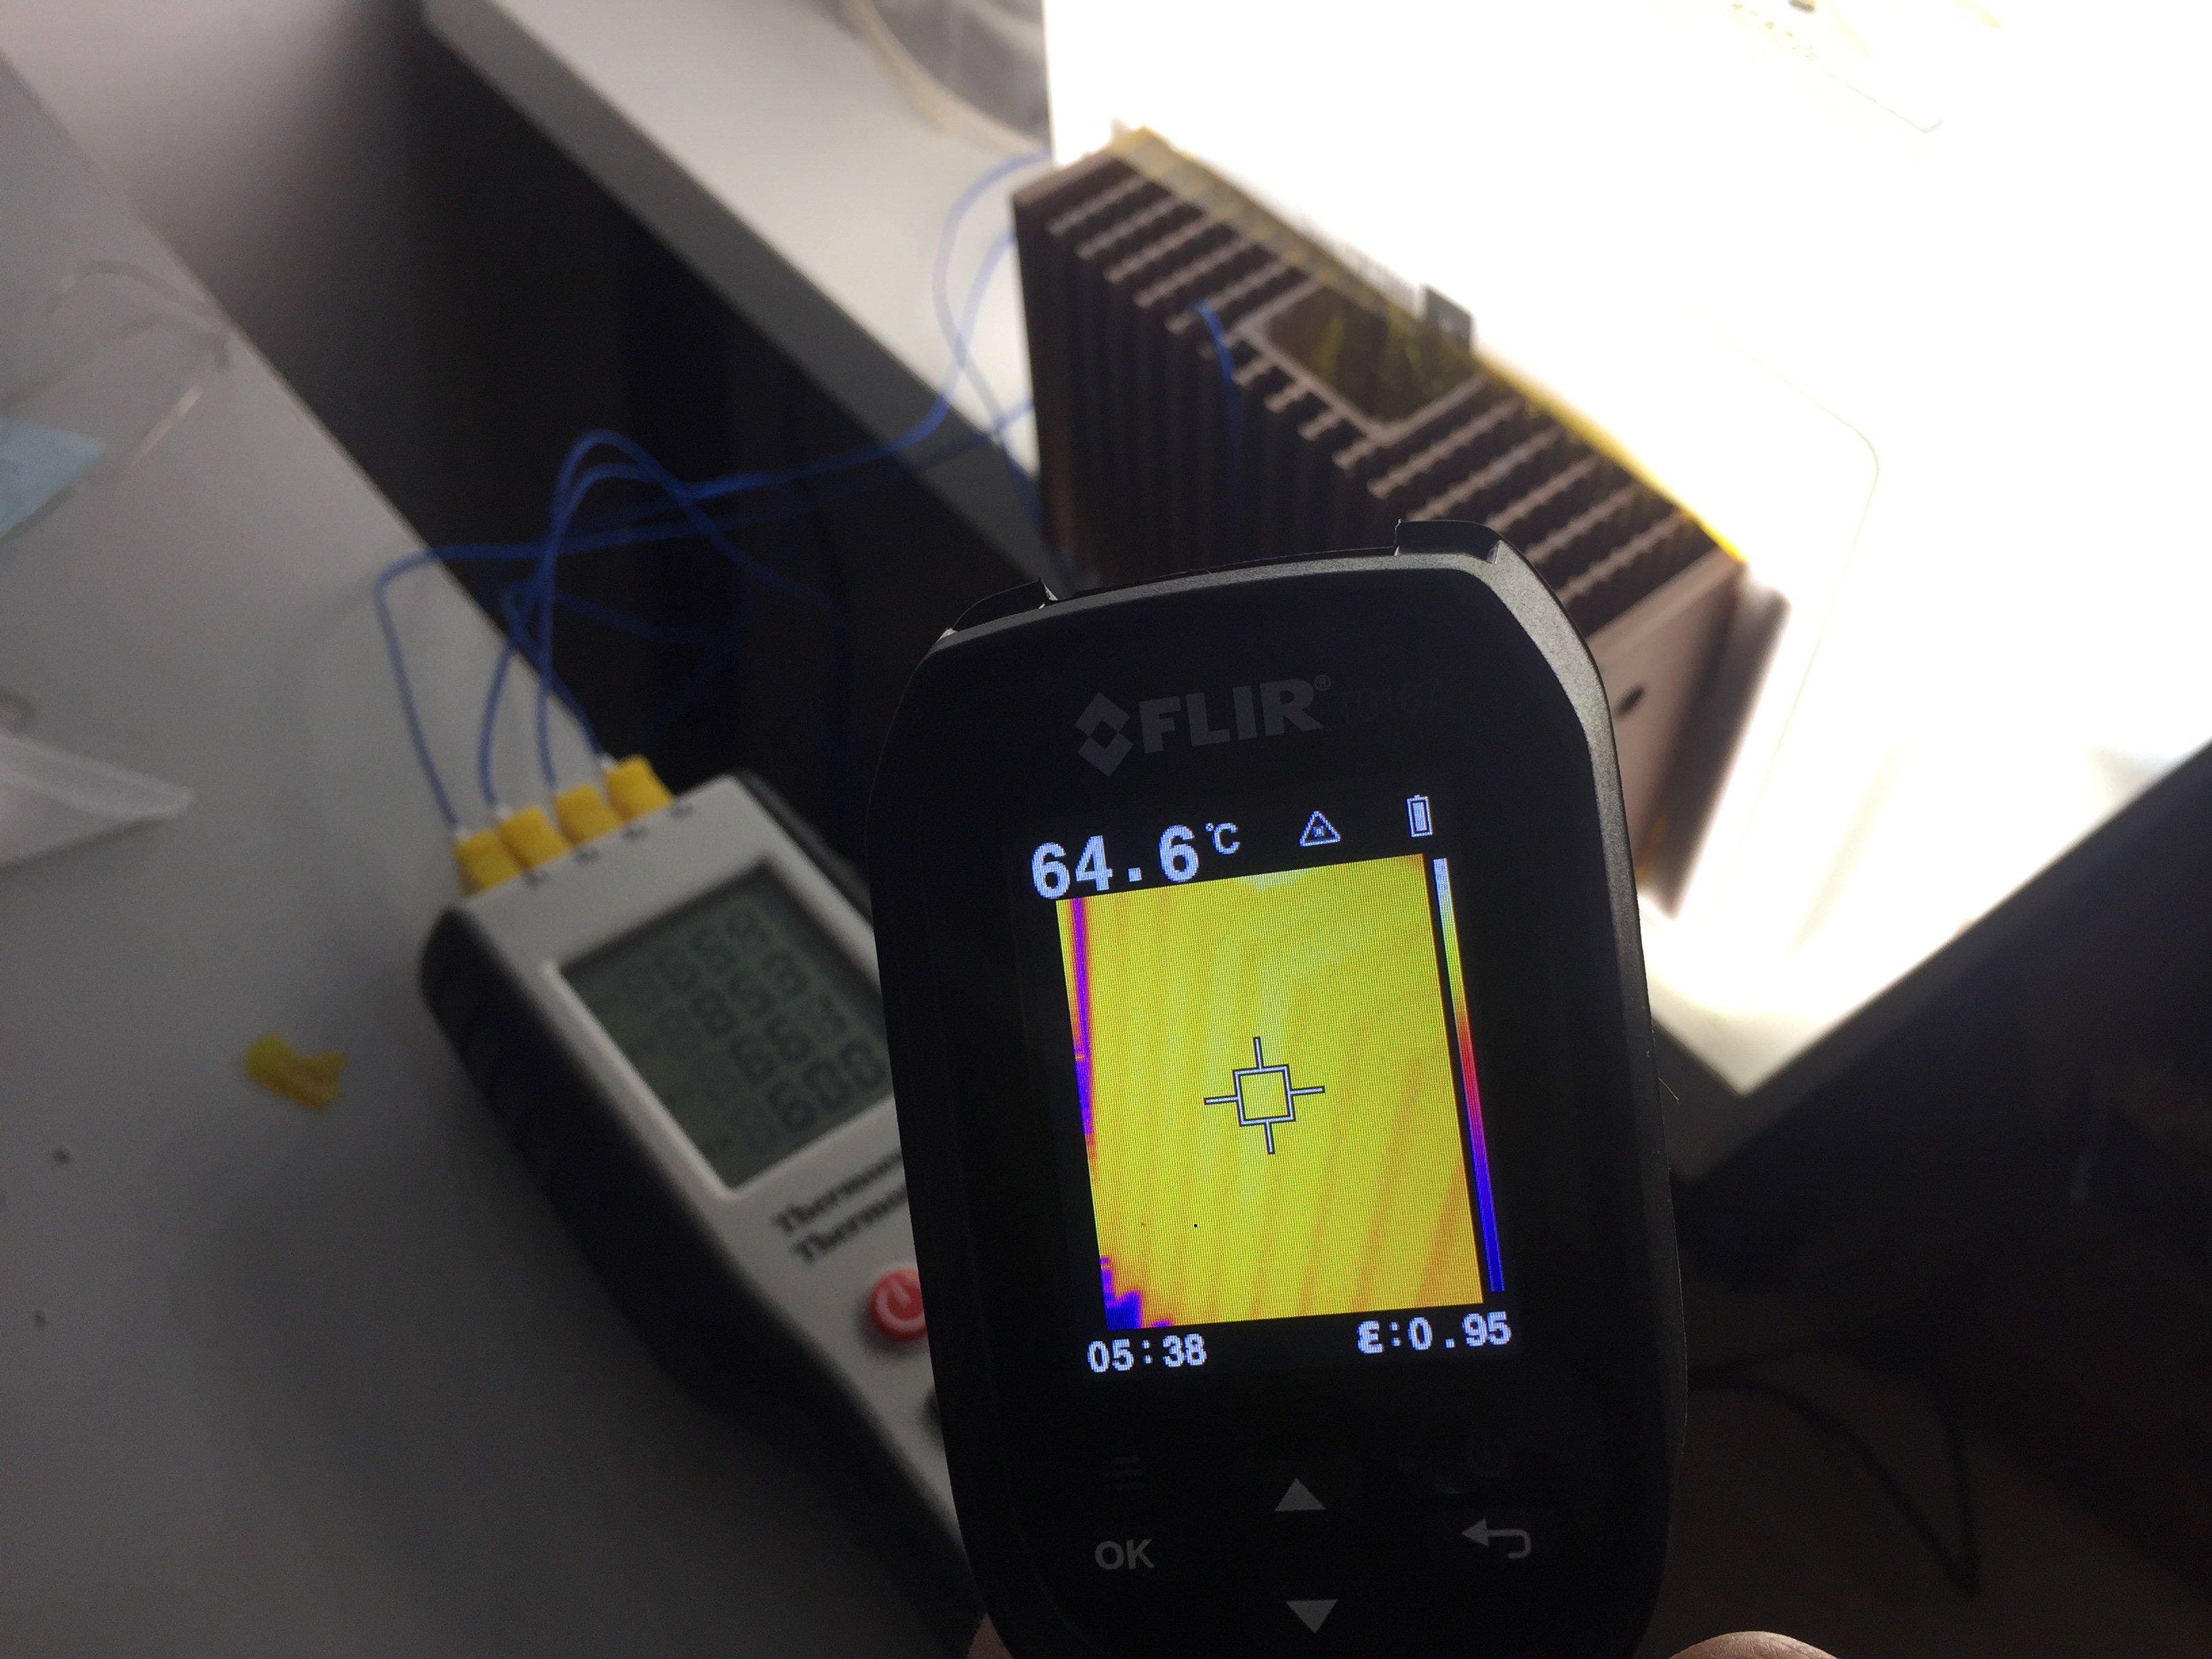
\includegraphics[scale=0.08]{figures/photos/thermal_camera.jpg}
\caption{Caméra thermique et sonde de température}
\label{fig:temp_test}
\end{figure}



\chapter{Apports}

A travers ce stage, j'ai approfondi mes connaissances dans de nombreux domaines : réseau, développement informatique, électronique embarquée, protocoles d'essais etc. Neohm étant une start-up avec peu d'employé, j'ai dû m'adapter au jour le jour aux besoins de l'entreprise et j'ai ainsi eu l'occasion de travailler sur divers projets. D'un point de vue culturel, ce stage m'a permis de découvrir un nouveau pays et une nouvelle culture. Travailler avec une équipe composée à la fois de Français et de Chinois a été une expérience très enrichissante. J'ai pu observer une manière différente d'aborder des problématiques et de trouver des solutions.

J'ai eu la chance d'avoir David comme tuteur. Avec son expérience de 20 ans dans cette région de Chine, il a su me guider tout au long de mon stage et m'aider à travailler avec des collègues chinois. Jean et Guillaume m'ont également fait partager leur attrait pour le marché chinois. Toute l'équipe de Neohm m'a très chaleureusement accueilli et m'a intégré rapidement.
Ce stage a été ma 1\ieme{} expérience longue en entreprise. Après mon installation et mon acclimatation qui ont duré environ 3 semaines, j'ai su me servir de mes connaissances et surtout de mon pragmatisme pour répondre aux problématiques des mes missions.

Ma rôle étant de programmer les microprocesseurs présents sur les circuits, j'ai renforcé mes connaissances du langage C et j'ai appris à construire un code robuste. J'ai dû appliqué des méthodes spécifiques à l'embarqué (utilisation d'interruptions par exemple) et adapter le code au hardware présent dans le circuit pour piloter certains contrôleurs et limiter la consommation électrique des composants.

Mes

\appendix

\chapter{Essais dans le laboratoire de lampe à LEDs}
\label{cha:labo_pictures}

\begin{figure}[H]
\centering
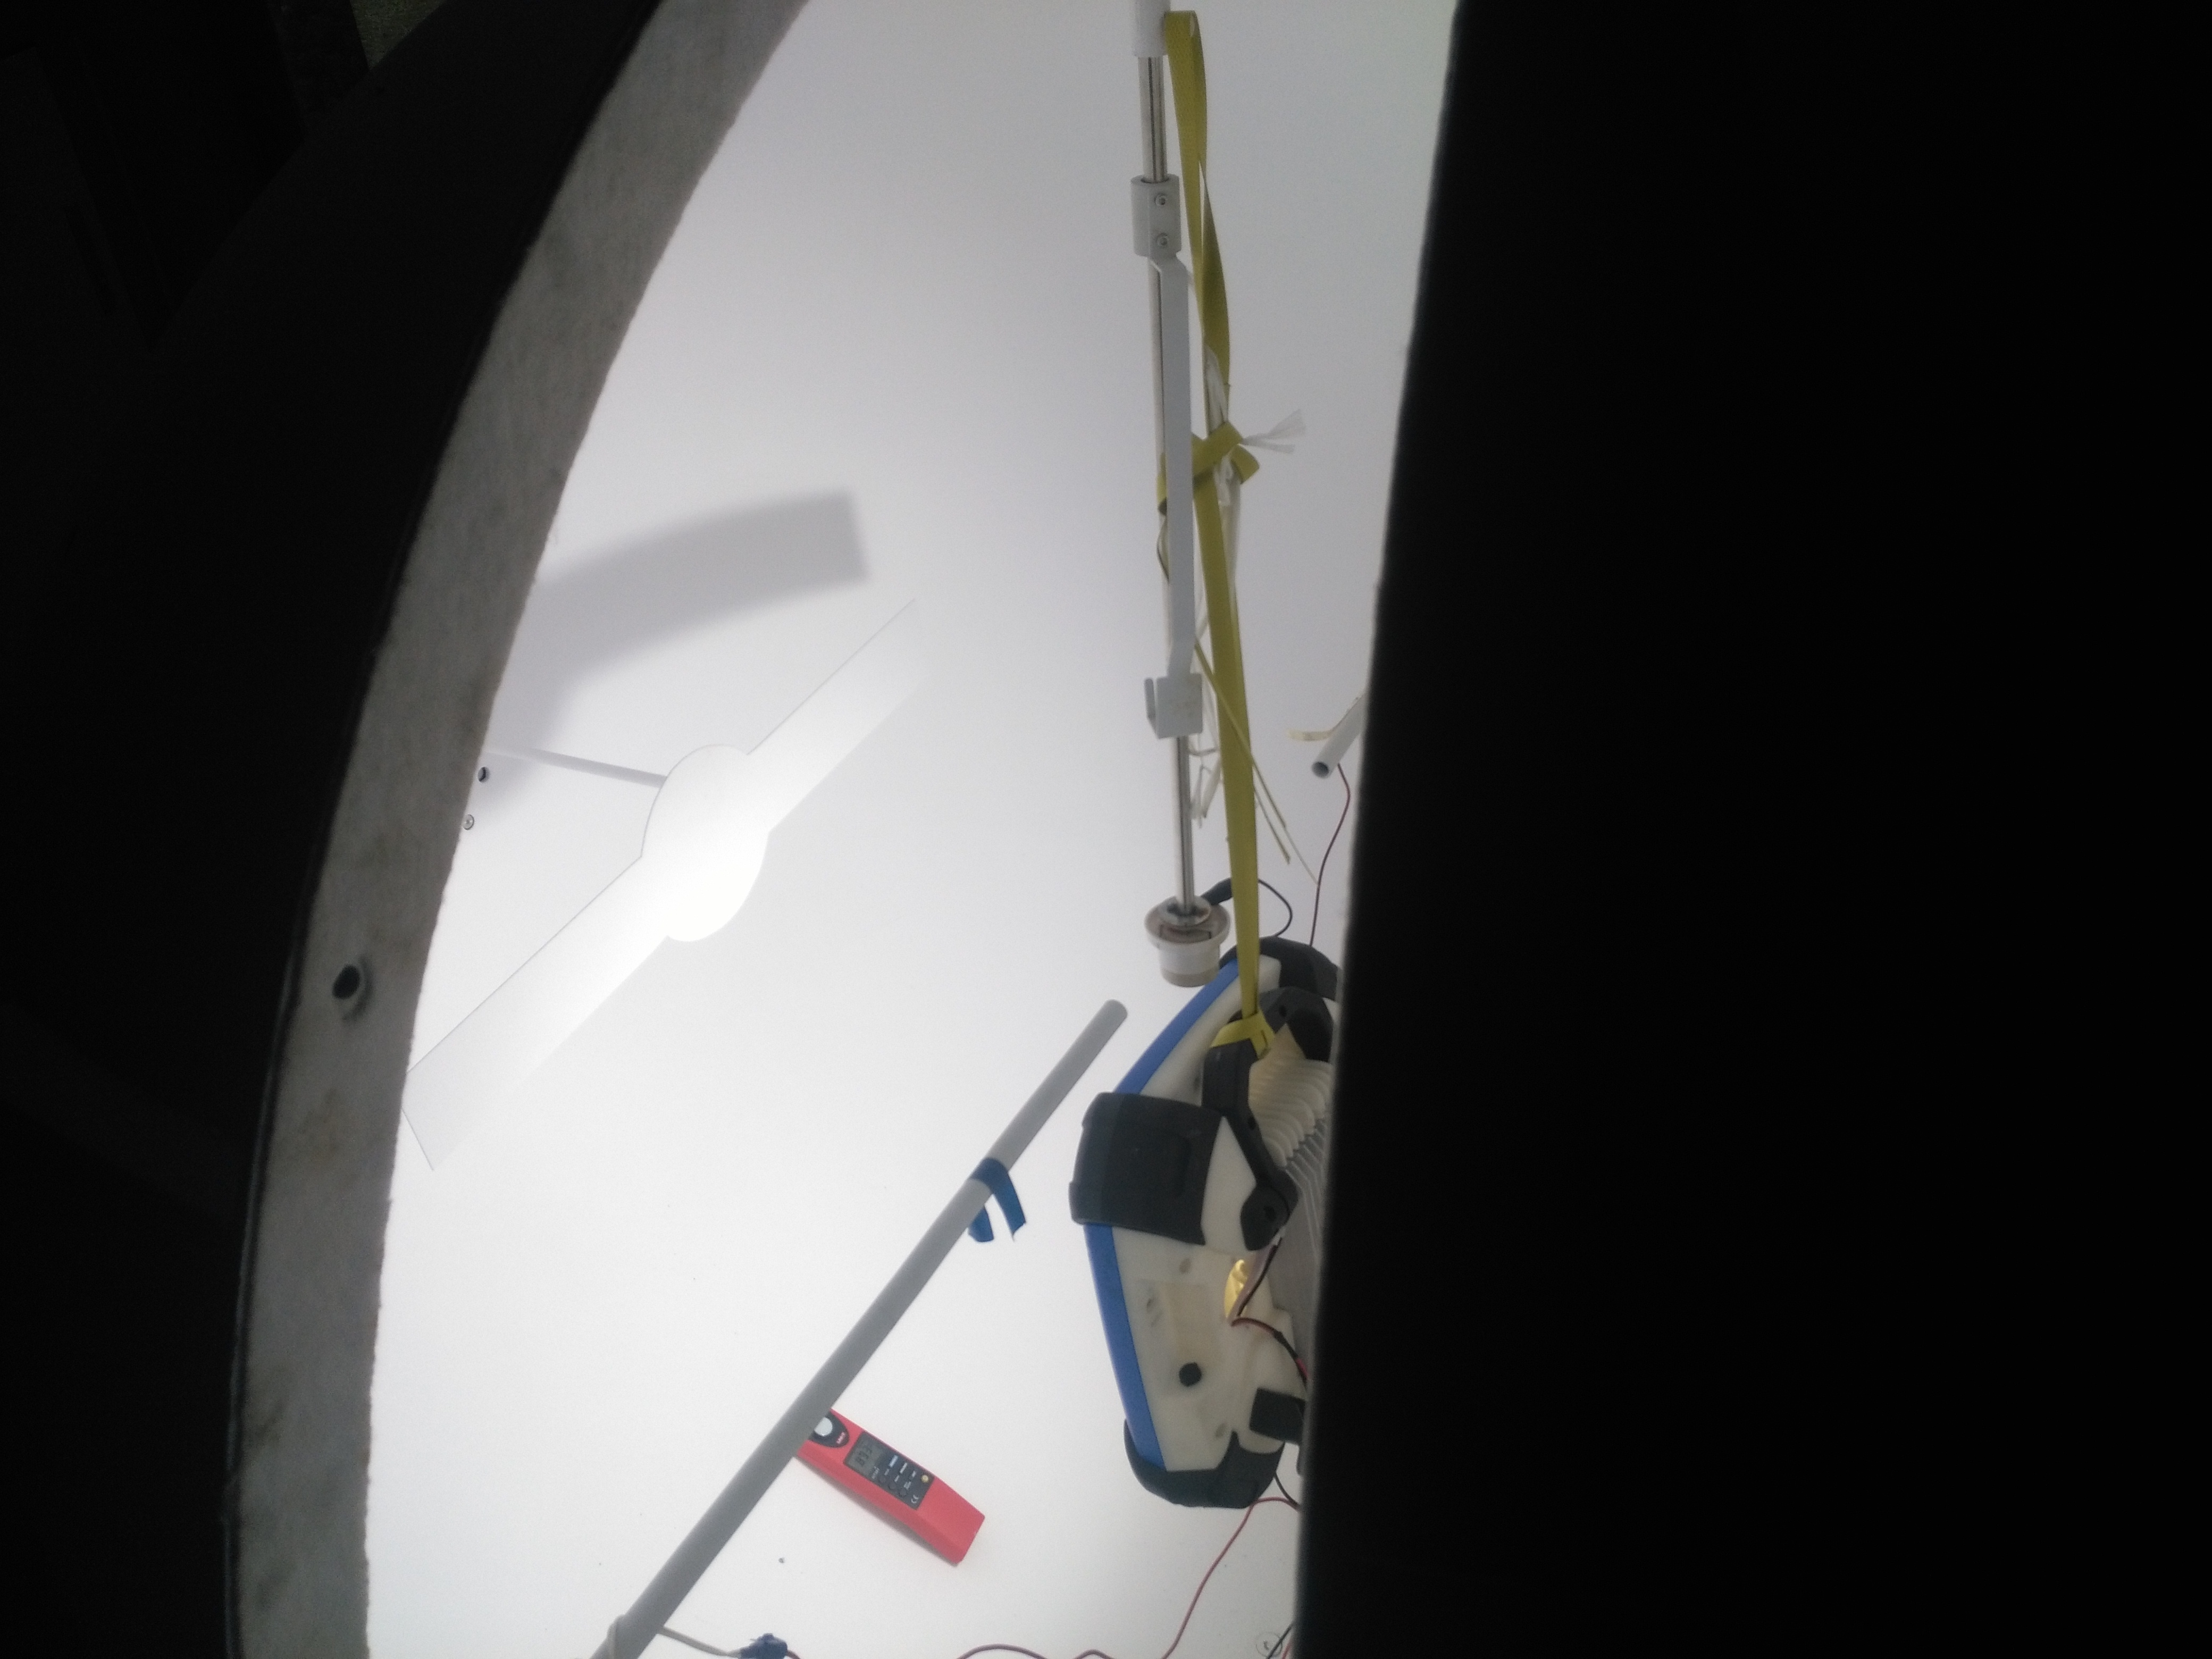
\includegraphics[scale=0.08]{figures/photos/tests_worklamp/sphere/sphere_allumee.jpg}
\caption{Sphère avec la lampe allumée} 
\label{fig:lamp_on}
\end{figure}

\begin{figure}[H]
\centering
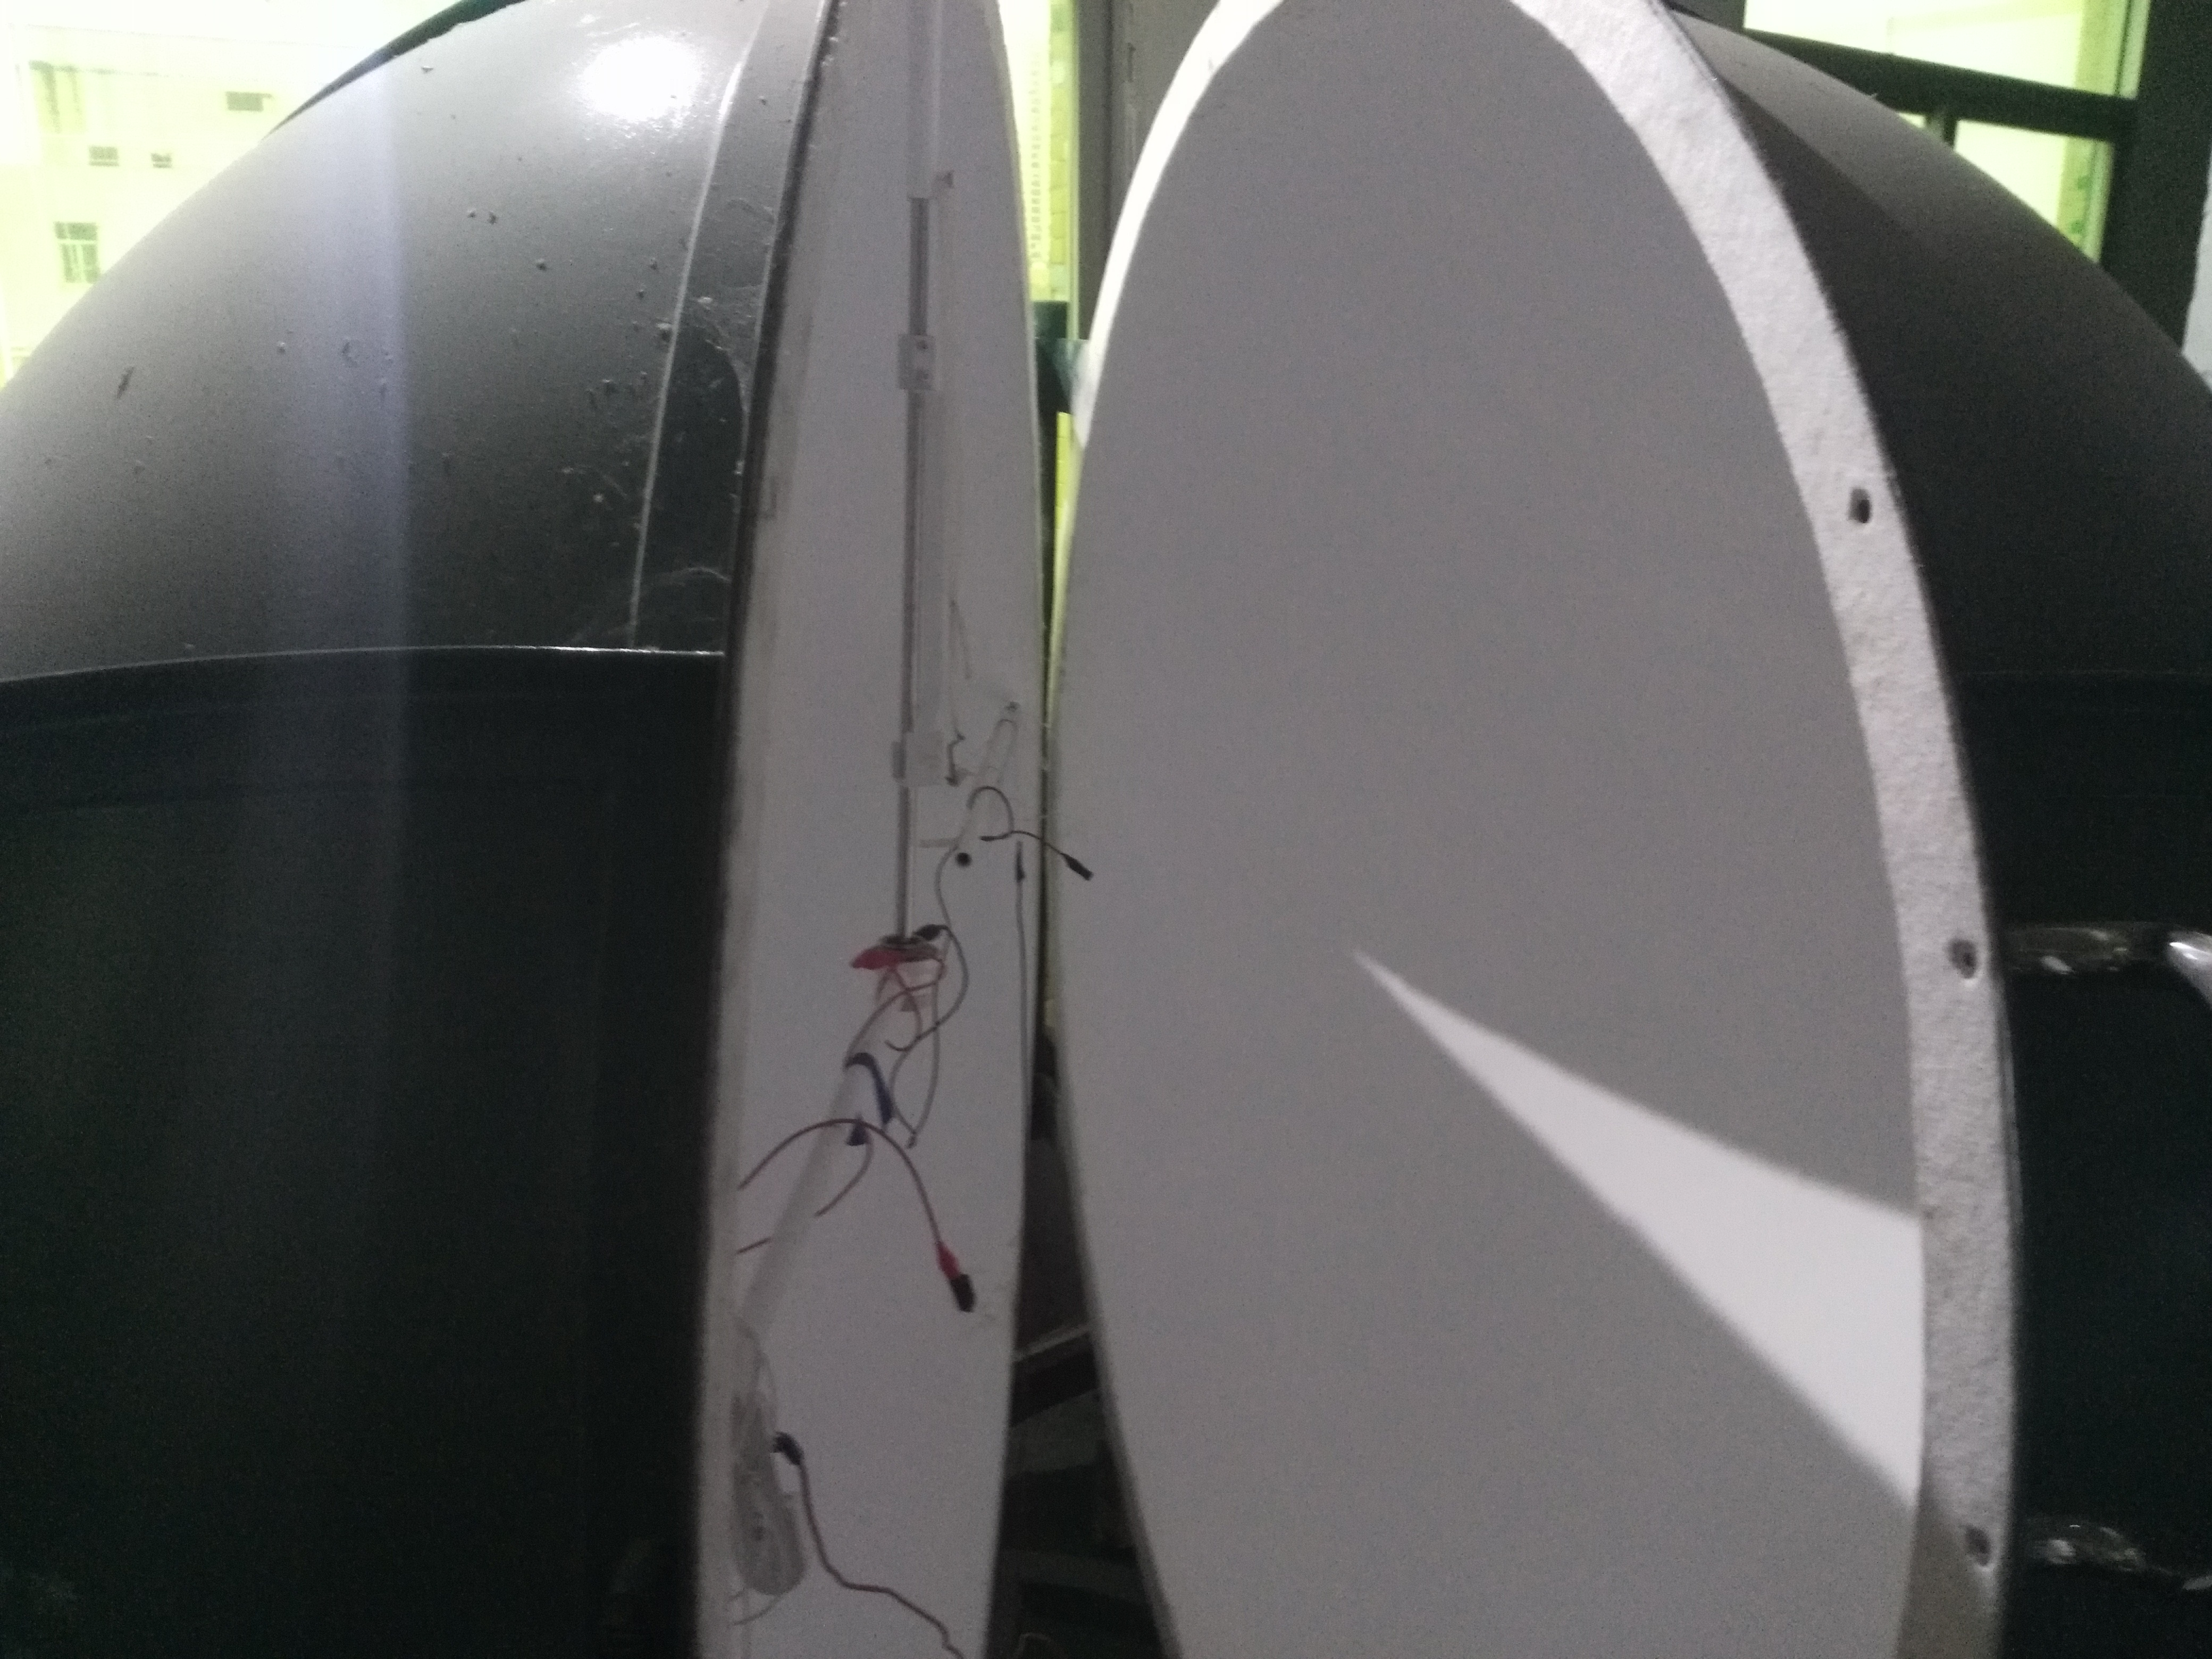
\includegraphics[scale=0.08]{figures/photos/tests_worklamp/sphere/spehre_vide.jpg}
\caption{Sphère intégrante vide}
\label{fig:empty_sphere}
\end{figure}

\begin{figure}[H]
\centering
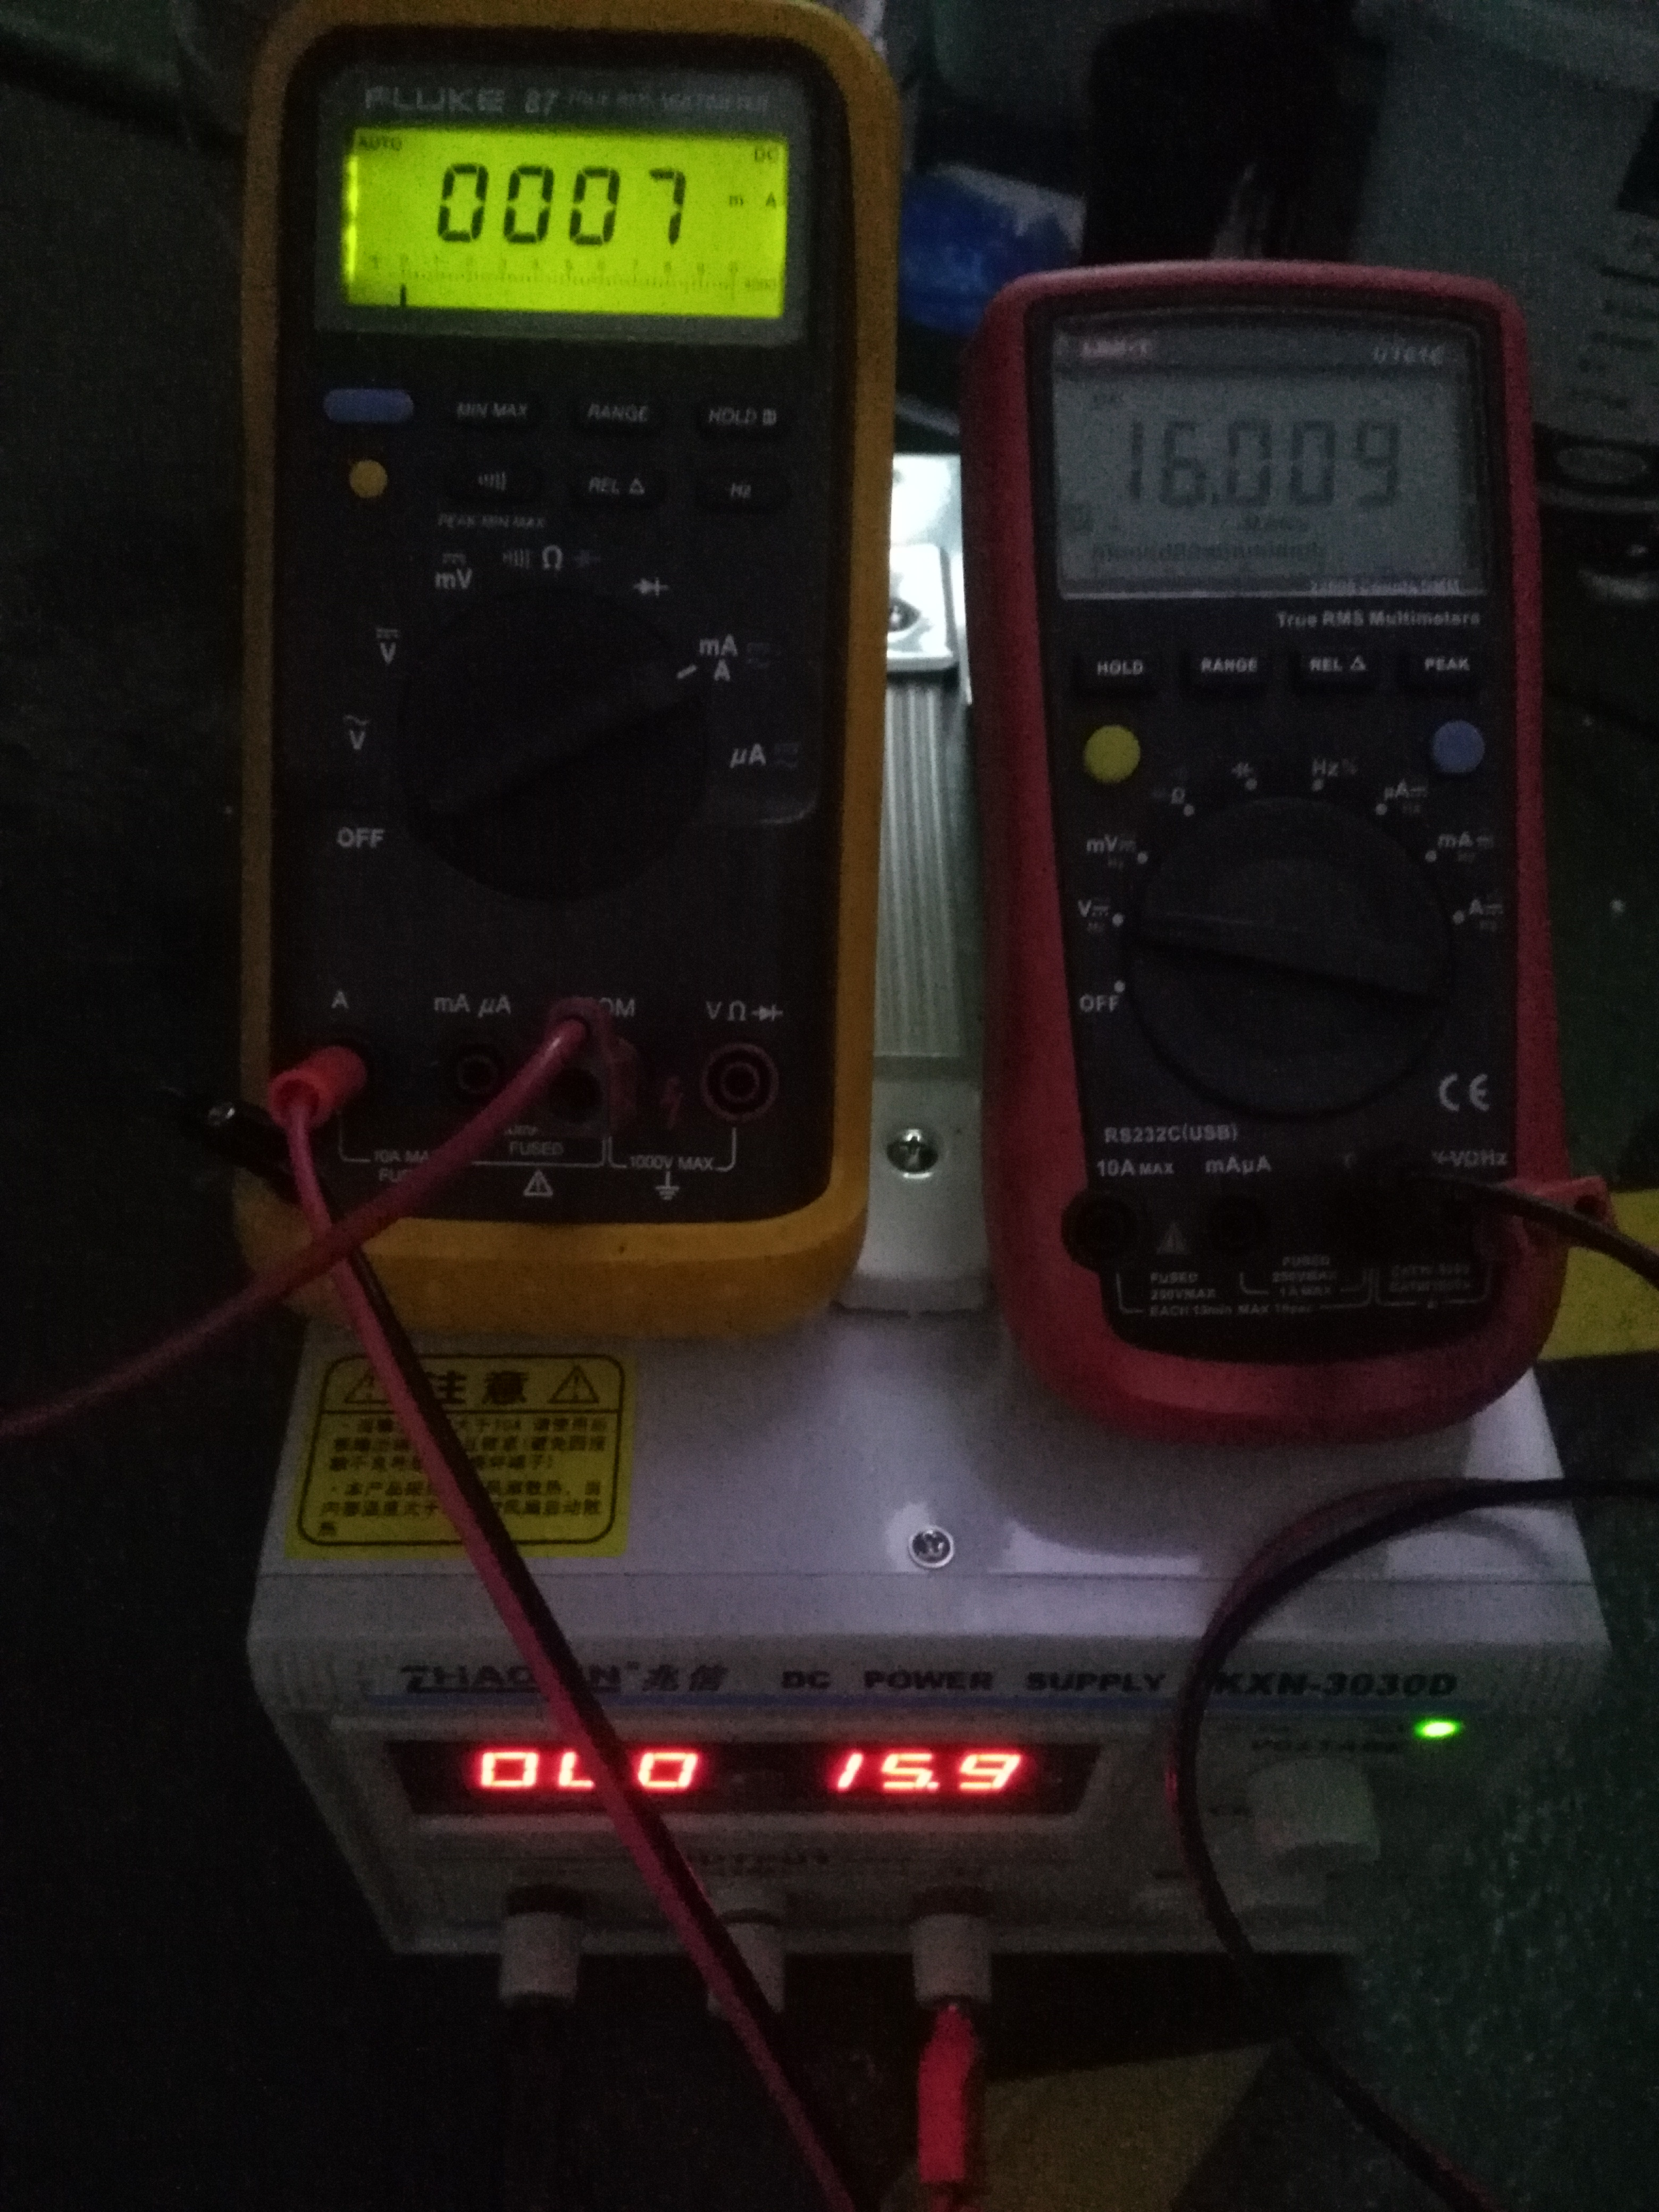
\includegraphics[scale=0.08]{figures/photos/tests_worklamp/sphere/mesure_1.jpg}
\caption{Générateur de tension et multimètre permettant de contrôler la lampe}
\label{fig:multimeters}
\end{figure}

\begin{figure}[H]
\centering
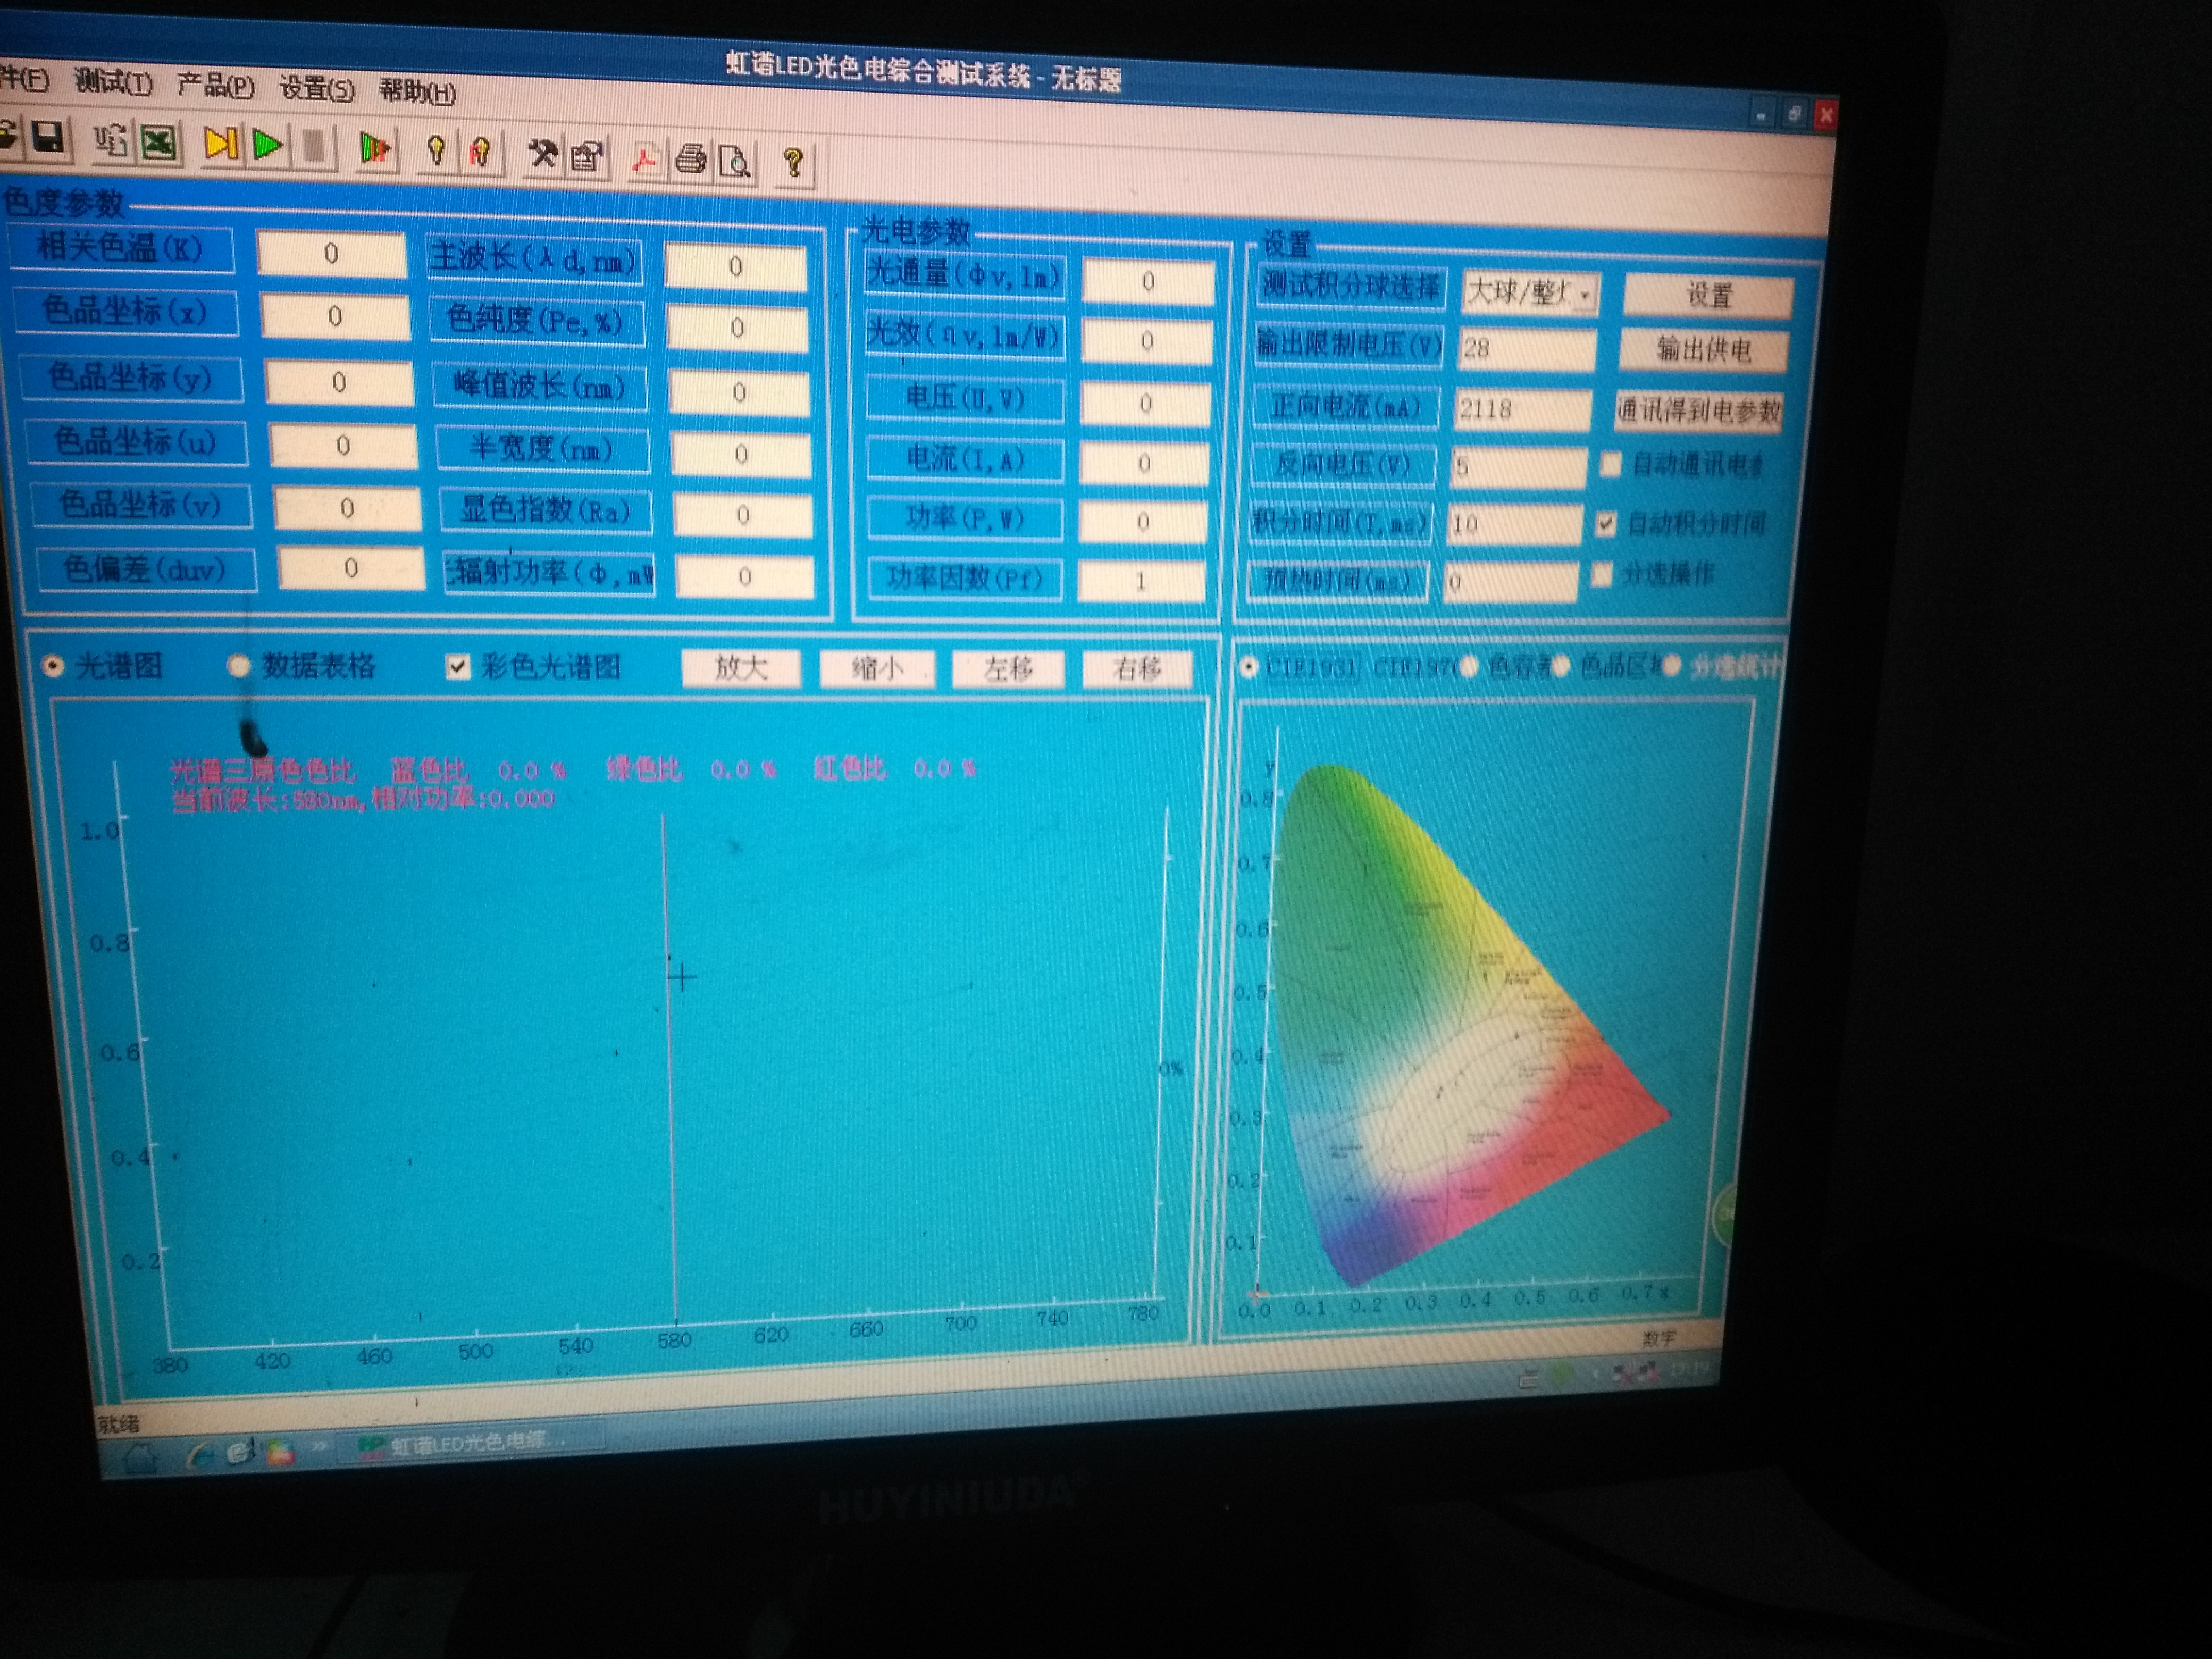
\includegraphics[scale=0.08]{figures/photos/tests_worklamp/sphere/ecran_PC.jpg}
\caption{Ecran du PC avec les résultats} 
\label{fig:PC_screen}
\end{figure}

\listoffigures

\bibliographystyle{plain}
\bibliography{bibli}

\end{document}